\chapter{拓扑空间}
\label{chap:topological-spaces}

在实轴上说“$x_n$趋于$x$”或“$f$在$x_0$处连续”，我们用的是距离：$\lvert x_n-x\rvert$能小于任意给定的正数，$\lvert x-x_0\rvert$足够小时$\lvert f(x)-f(x_0)\rvert$也足够小。

细看这些定义，真正起作用的是“$x$附近”的一组区域，距离的具体数值并不重要：$x_n$最终落进$x$附近的每个区间，$f$把$x_0$附近的某个区间送进$f(x_0)$附近的给定区间。圆周、曲面、函数的集合以及粘合而成的空间上，往往没有现成的、唯一合适的距离，却仍然需要谈论“附近”“趋于”和“连续”。

本章把“附近”从距离中分离出来，用开集族作为唯一的基本数据。第~\ref{sec:topo-topology}节从实轴开区间满足的规则得到拓扑的定义，并用拓扑基与邻域基描述全部开集和一个点附近的区域。第~\ref{sec:topo-subsets}节考察子集与环境空间的关系，第~\ref{sec:topo-convergence}节研究点列，第~\ref{sec:topo-continuous-maps}节研究空间之间的映射。

第~\ref{sec:topo-constructions}节用子集、乘积和粘合造出新空间，每种构造都由“哪些映射应当连续”确定新的开集。第~\ref{sec:topo-properties}节集中讨论空间本身的性质：不同点能否被分开，开集与邻域能否用可数个代表描述，空间能否拆成两块，开覆盖能否化为有限个。

本章始终不使用距离。点到集合的距离、序列判据、完备性以及紧性的序列判据属于第~\ref{chap:metric-spaces}章，连续映射的距离判据、均匀连续与映射列的收敛属于第~\ref{chap:metric-space-maps}章。乘积空间为第~\ref{chap:homology}章的同伦准备定义域，分离性、可数性、连通性与紧性是第~\ref{chap:manifold-basics}章定义流形时要核验的条件。

\section{拓扑的定义}
\label{sec:topo-topology}

要在一个集合上谈论“附近”，需要规定哪些子集算作“围住其中每一点”的区域。本节从实轴上的开集总结出这类区域应满足的规则，把满足规则的子集族定义为拓扑，再说明怎样用较小的子集族生成全部开集，以及怎样只看一个点周围的区域。

\subsection{开集}
\label{sec:topo-open-sets}

开区间$(a,b)$有一个直观特点：它的每个点两侧都还留有余地，稍微移动一点仍在区间内。闭区间$[a,b]$的端点$a$没有这种余地，向左移动任意一点就离开了区间。把“留有余地”写成要求，就得到实轴上开集的概念。

\paragraph{实轴上的开集}
集合$U\subseteq\mathbb R$称为开集，如果对每个$x\in U$都存在$r>0$，使$(x-r,x+r)\subseteq U$。这里的半径$r$可以随$x$改变，越靠近边缘的点，能取的半径越小。

以$U=(0,1)\cup(2,3)$为例，取其中的点$x=2.9$。它到所在区间两端的距离分别是$0.9$与$0.1$，取较小者
\[
 r=\min\{2.9-2,\ 3-2.9\}=0.1,
\]
就有$(2.8,3)\subseteq U$。每个点都能这样取半径，所以$U$是开集。

$[0,1)$不是开集。问题只出在点$0$：无论$r>0$多小，$(-r,r)$都含有负数。卷一已经用这一定义讨论过闭集的序列判据和闭区间的有限子覆盖性质，可参考\BookChapterRef{chap:limits-continuity}{卷一第5章“极限与连续”}。这里关心的是开集族作为一个整体满足什么规则。

\begin{lemma}[实轴开集的运算规则]
\label{lem:topo-real-open-rules}
实轴上的开集满足：
\begin{enumerate}
  \item $\varnothing$与$\mathbb R$是开集；
  \item 任意一族开集的并是开集；
  \item 有限个开集的交是开集。
\end{enumerate}
\end{lemma}
\begin{proof}
空集没有点，条件自动成立。对$\mathbb R$的每个点取$r=1$，就得到$\mathbb R$是开集。

设$\{U_i\}_{i\in I}$是一族开集，$x\in\bigcup_iU_i$。则$x$属于某个$U_{i_0}$，存在$r>0$使
\[
 (x-r,x+r)\subseteq U_{i_0}\subseteq\bigcup_iU_i.
\]

设$U_1,\dots,U_k$是开集，$x\in U_1\cap\cdots\cap U_k$。对每个$j$取$r_j>0$使$(x-r_j,x+r_j)\subseteq U_j$，并令
\[
 r=\min\{r_1,\dots,r_k\}.
\]
只有有限个正数，所以$r>0$。区间$(x-r,x+r)$含于每个$U_j$，从而含于它们的交。
\end{proof}

第三条中的“有限”不能去掉。开区间$(-1/n,1/n)$（$n=1,2,\dots$）都含$0$，它们的交是单点集：
\[
 \bigcap_{n\geq1}\Bigl(-\frac1n,\frac1n\Bigr)=\{0\},
\]
而$\{0\}$不是开集。证明中失效的正是取最小值这一步：无限多个半径$1/n$的下确界为$0$，取不到一个对所有区间都适用的正半径。

\paragraph{拓扑}
引理~\ref{lem:topo-real-open-rules}的三条规则不涉及区间长度，只涉及集合的并与交。把它们作为公理，就能在任何集合上规定“开集”。

\begin{definition}[拓扑与拓扑空间]
\label{def:topo-topology}
设$X$是集合，$\mathcal T$是$X$的一族子集。若
\begin{enumerate}
  \item $\varnothing\in\mathcal T$，$X\in\mathcal T$；
  \item $\mathcal T$中任意多个成员的并仍属于$\mathcal T$；
  \item $\mathcal T$中有限多个成员的交仍属于$\mathcal T$，
\end{enumerate}
则称$\mathcal T$为$X$上的一个\term{拓扑}（topology），称$(X,\mathcal T)$为\term{拓扑空间}（topological space），称$\mathcal T$的成员为\term{开集}（open set）。
\end{definition}

可以把$\mathcal T$看作一份清单：它列出$X$中哪些子集被认可为“围得住其中各点”的区域。向量空间的定义规定了向量能怎样相加，却不规定向量是什么；拓扑的定义同样只规定清单要满足的封闭性，不规定开集长什么样。

不致混淆时，我们直接说“拓扑空间$X$”。第三条只需对两个集合验证：若$U,V\in\mathcal T$时总有$U\cap V\in\mathcal T$，对个数归纳就得到有限交。由引理~\ref{lem:topo-real-open-rules}确定的开集族称为$\mathbb R$的\term{通常拓扑}（standard topology），以后提到$\mathbb R$而不另加说明时，都指这个拓扑。

有限集上的拓扑可以逐个集合核对，是检验定义的好材料。图~\ref{fig:topo-finite-topologies}在三点集$X=\{a,b,c\}$上画了三份清单，每条闭曲线圈出清单中的一个集合。

\begin{BookInlineFigure}
  \centering
  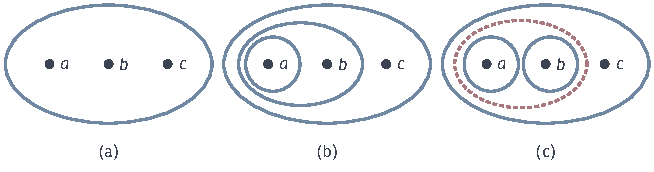
\includegraphics[width=110.786mm]{figures/04-spaces-measures-and-geometry/01-topology-and-metric/tikz/topo-finite-topologies/figure.pdf}
  \caption{三点集$X=\{a,b,c\}$上的三个子集族，每条蓝色闭曲线圈出族中的一个集合，空集未画出。(a)只有$X$，是拓扑。(b)$\{a\}$、$\{a,b\}$、$X$层层嵌套，是拓扑。(c)有$\{a\}$与$\{b\}$却缺少它们的并$\{a,b\}$（红色虚线），不是拓扑。}
  \label{fig:topo-finite-topologies}
\end{BookInlineFigure}

图(b)对应的族是
\[
 \mathcal T=\bigl\{\varnothing,\ \{a\},\ \{a,b\},\ X\bigr\}.
\]
它的成员依次包含，任取两个，并是较大的那个，交是较小的那个，结果都还在族中，所以$\mathcal T$是拓扑。图(c)的族含有$\{a\}$和$\{b\}$，它们的并$\{a,b\}$却不在族中，并封闭这一条不成立。

\paragraph{同一集合上的不同拓扑}
拓扑是附加在集合上的结构，同一个集合可以配上很不相同的拓扑。两个极端情形最能说明这一点。

\begin{example}[离散拓扑与平凡拓扑]
\label{ex:topo-discrete-indiscrete}
对任意集合$X$，全部子集组成的族$\mathcal P(X)$满足定义~\ref{def:topo-topology}，称为\term{离散拓扑}（discrete topology）。这时每个单点集$\{x\}$都是开集，$x$附近只有它自己。

另一端是$\{\varnothing,X\}$，它也满足三条规则，称为\term{平凡拓扑}（indiscrete topology）。这时唯一包含$x$的开集是整个$X$，空间中任何两点都无法用开集区分。

在两点集$X=\{a,b\}$上，$\{\varnothing,\{a\},X\}$也是拓扑。包含$b$的开集只有$X$，它也包含$a$；$a$却有一个不含$b$的开集$\{a\}$。在这个拓扑下，$a$总在$b$的每个开集里，反过来却不成立，“附近”这一关系可以不对称。
\end{example}

清单越长，可用来围住点的区域越多，点与点之间就越能区分。设$\mathcal T_1\subseteq\mathcal T_2$是同一集合上的两个拓扑，称$\mathcal T_2$比$\mathcal T_1$\term{更细}（finer），$\mathcal T_1$比$\mathcal T_2$更粗。

离散拓扑最细，平凡拓扑最粗，$\mathbb R$的通常拓扑介于二者之间。两个拓扑也可以互不包含：在$\{a,b\}$上，$\{\varnothing,\{a\},X\}$与$\{\varnothing,\{b\},X\}$就谈不上谁更细。

\subsection{拓扑基}
\label{sec:topo-basis}

实轴的开集可以形状复杂，例如$\bigcup_{n\geq1}(1/(n+1),1/n)$，但每个开集都是若干开区间的并：对开集$U$的每个点$x$取一个含于$U$的区间$(x-r_x,x+r_x)$，这些区间的并恰好是$U$。只要知道“开区间”这一小类集合，就能确定全部开集。

这与线性空间中用基表示向量相似：基向量通过线性组合得到所有向量，基本开集通过取并得到所有开集。类比到这里为止，因为取并没有系数，表示方式一般也不唯一，“基”的成员之间也不要求任何独立性。

\begin{definition}[拓扑基]
\label{def:topo-basis}
设$(X,\mathcal T)$是拓扑空间，$\mathcal B\subseteq\mathcal T$。若每个开集都能写成$\mathcal B$中若干成员的并，就称$\mathcal B$为$\mathcal T$的一个\term{拓扑基}（basis for a topology），$\mathcal B$的成员称为基本开集。
\end{definition}

空集是$\mathcal B$中零个成员的并，所以这一要求对空集自动成立。判断一个开集族是否为拓扑基时，逐点检验往往更方便：$\mathcal B\subseteq\mathcal T$是拓扑基，当且仅当对每个开集$U$和每个$x\in U$，都存在$B\in\mathcal B$使
\begin{equation}
 x\in B\subseteq U.
 \label{eq:topo-basis-pointwise}
\end{equation}

必要性是因为$x$属于表示$U$的某个成员。充分性是因为把这些$B$对$x\in U$取并，得到的集合含于$U$，又包含$U$的每个点，所以恰好等于$U$。图~\ref{fig:topo-basis-criterion}(a)画的就是这个判据：靠近边缘的点只是需要更小的基本开集。

\paragraph{由一族集合生成拓扑}
在欧氏空间里，我们往往先想到一类形状简单的集合，再希望用它们生成拓扑。这时需要判断：一族子集在什么条件下能作为某个拓扑的基。

\begin{theorem}[生成拓扑的基]
\label{thm:topo-basis-criterion}
设$X$是集合，$\mathcal B$是$X$的一族子集，满足
\begin{enumerate}
  \item $\mathcal B$的成员覆盖$X$，即每个$x\in X$都属于某个$B\in\mathcal B$；
  \item 若$x\in B_1\cap B_2$，$B_1,B_2\in\mathcal B$，则存在$B_3\in\mathcal B$使$x\in B_3\subseteq B_1\cap B_2$。
\end{enumerate}
令$\mathcal T$为$\mathcal B$中成员的所有并组成的族，则$\mathcal T$是$X$上的拓扑，$\mathcal B$是它的拓扑基。反过来，任何拓扑的拓扑基都满足这两条。
\end{theorem}
\begin{proof}
空集是零个成员的并，由条件1，$X$是全部成员的并，所以$\varnothing,X\in\mathcal T$。若干个“$\mathcal B$中成员的并”再取并，仍是$\mathcal B$中成员的并，所以$\mathcal T$对任意并封闭。

剩下验证两个集合的交。设$U=\bigcup_iB_i$，$V=\bigcup_jB'_j$，$x\in U\cap V$。则存在一对$i,j$使$x\in B_i\cap B'_j$，由条件2可取$B_x\in\mathcal B$，使
\[
 x\in B_x\subseteq B_i\cap B'_j\subseteq U\cap V.
\]
对$x\in U\cap V$取并，得到
\[
 U\cap V=\bigcup_{x\in U\cap V}B_x\in\mathcal T.
\]

反过来，设$\mathcal B$是拓扑$\mathcal T$的基。$X$是开集，必是$\mathcal B$中成员的并，条件1成立。$B_1\cap B_2$是开集，把判据\eqref{eq:topo-basis-pointwise}用于它，就得到条件2。
\end{proof}

条件2的作用可以从图~\ref{fig:topo-basis-criterion}(b)看出：两个基本开集的交不必本身是基本开集，但在交的每个点处都要放得下一个基本开集。

\begin{BookInlineFigure}
  \centering
  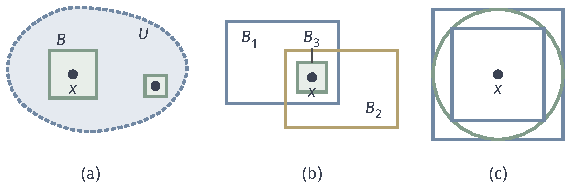
\includegraphics[width=96.227mm]{figures/04-spaces-measures-and-geometry/01-topology-and-metric/tikz/topo-basis-criterion/figure.pdf}
  \caption{拓扑基的三个判断。(a)开集$U$（虚线边界）中的每个点都有一个含于$U$的基本开集（绿色），靠近边界的点需要更小的方块。(b)定理条件2：在$B_1\cap B_2$的点$x$处放得下基本开集$B_3$。(c)以$x$为中心，正方形、圆盘、更小的正方形依次嵌套，所以方块与圆盘生成同样的开集。}
  \label{fig:topo-basis-criterion}
\end{BookInlineFigure}

条件2不能省略。在$X=\{a,b,c\}$上取$\mathcal B=\{\{a,b\},\{b,c\}\}$，它覆盖$X$。两个成员的交是$\{b\}$，而$\mathcal B$中没有成员能放进$\{b\}$，条件2不成立。所有的并组成的族是
\[
 \bigl\{\varnothing,\ \{a,b\},\ \{b,c\},\ X\bigr\},
\]
它不含$\{a,b\}\cap\{b,c\}=\{b\}$，的确不是拓扑。

\begin{example}[开区间与开矩形]
\label{ex:topo-intervals-rectangles}
全体开区间$(a,b)$构成$\mathbb R$通常拓扑的基，这正是本小节开头的观察。

在平面$\mathbb R^2$上，取全体开矩形$(a_1,b_1)\times(a_2,b_2)$组成的族$\mathcal B$。它覆盖$\mathbb R^2$，两个开矩形的交为
\[
\begin{aligned}
&\bigl((a_1,b_1)\times(a_2,b_2)\bigr)\cap\bigl((c_1,d_1)\times(c_2,d_2)\bigr)\\
&\qquad=\bigl((a_1,b_1)\cap(c_1,d_1)\bigr)\times\bigl((a_2,b_2)\cap(c_2,d_2)\bigr).
\end{aligned}
\]
两个开区间的交是开区间或空集，所以这个交仍是开矩形或空集，条件2成立。

由定理~\ref{thm:topo-basis-criterion}，开矩形生成$\mathbb R^2$上的一个拓扑，称为$\mathbb R^2$的通常拓扑。$\mathbb R^n$上用$n$个开区间的乘积同样处理。
\end{example}

不同的基可以生成同一个拓扑。在$\mathbb R^2$上改用全体开圆盘作基，条件1、2同样成立。如图~\ref{fig:topo-basis-criterion}(c)，圆盘内任一点周围都能放进一个以它为中心的小正方形，正方形内任一点周围也能放进一个小圆盘。由判据\eqref{eq:topo-basis-pointwise}，两族集合生成的开集完全相同，开集并不取决于用正方形还是圆形去度量附近。

\subsection{邻域}
\label{sec:topo-neighborhoods}

讨论一个点附近的性质时，用到的区域不必恰好是开集。要说“$f$在$x=1/2$附近取正值”，说它在$[0,1]$上取正值就够了，尽管$[0,1]$不是开集。关键在于这个集合包含一个围住$1/2$的开集。

\begin{definition}[邻域]
\label{def:topo-neighborhood}
设$X$是拓扑空间，$x\in X$。若集合$N\subseteq X$包含某个开集$U$，且$x\in U$，就称$N$是$x$的\term{邻域}（neighborhood）。本身是开集的邻域称为\term{开邻域}（open neighborhood）。
\end{definition}

在$\mathbb R$中，$[0,1]$是$1/2$的邻域，因为它包含开集$(1/4,3/4)\ni1/2$。它不是$0$的邻域，因为包含$0$的任何开集都含有负数，见图~\ref{fig:topo-neighborhoods}(a)。这说明两点：邻域本身不必是开集；“是邻域”总是相对于某个指定点而言，同一个集合可以是某些点的邻域而不是另一些点的邻域。

\begin{BookInlineFigure}
  \centering
  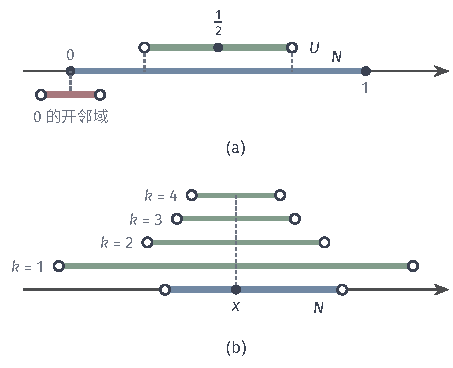
\includegraphics[width=76.793mm]{figures/04-spaces-measures-and-geometry/01-topology-and-metric/tikz/topo-neighborhoods/figure.pdf}
  \caption{邻域与邻域基。(a)蓝色的$N=[0,1]$包含绿色开集$U=(1/4,3/4)$，因此是$1/2$的邻域；$0$的任一开邻域（红色）都伸出$N$之外，所以$N$不是$0$的邻域。(b)绿色区间是$(x-1/k,x+1/k)$，蓝色区间是邻域$N=(x-0.4,x+0.6)$；$k=3$的区间已经含于$N$。}
  \label{fig:topo-neighborhoods}
\end{BookInlineFigure}

邻域与开集的关系可以反过来刻画开集：开集正是“对自己的每个点都是邻域”的集合。

\begin{lemma}[开集的邻域刻画]
\label{lem:topo-open-iff-neighborhood}
集合$U\subseteq X$是开集，当且仅当$U$是它的每个点的邻域。
\end{lemma}
\begin{proof}
若$U$开，对每个$x\in U$，$U$本身就是含$x$且含于$U$的开集。

反过来，若对每个$x\in U$都有开集$U_x$满足$x\in U_x\subseteq U$，则
\[
 U=\bigcup_{x\in U}U_x.
\]
拓扑对任意并封闭，所以$U$是开集。
\end{proof}

实轴开集的原始定义“每点两侧留有余地”正是这个引理的特例。以后证明一个集合是开集，常用的办法就是逐点找到含于其中的开邻域。

\subsection{邻域基}
\label{sec:topo-neighborhood-basis}

判断实数列$x_n\to x$时，并不需要检验$x$的所有邻域，只需检验区间$(x-1/k,x+1/k)$，$k=1,2,\dots$，因为任何邻域都包含其中某一个。这类足以代表所有邻域的子族，是描述一个点附近最经济的工具。

\begin{definition}[邻域基]
\label{def:topo-neighborhood-basis}
设$x\in X$，$\mathcal B_x$是$x$的一族邻域。若$x$的每个邻域$N$都包含$\mathcal B_x$中的某个成员，就称$\mathcal B_x$是$x$的\term{邻域基}（neighborhood basis）。
\end{definition}

在$\mathbb R$中，$\{(x-1/k,x+1/k):k\geq1\}$是$x$的邻域基。给定$x$的邻域$N$，它包含某个开集$U\ni x$，而$U$又包含某个$(x-r,x+r)$。取$k>1/r$，就有
\[
 \Bigl(x-\frac1k,x+\frac1k\Bigr)\subseteq(x-r,x+r)\subseteq N.
\]

图~\ref{fig:topo-neighborhoods}(b)是一个具体的情形：$N=(x-0.4,x+0.6)$的左侧余量是$0.4$，右侧余量是$0.6$，可取$r=0.4$。$k=2$时半径$0.5$超过左侧余量，$k=3$时半径$1/3<0.4$，区间已经含于$N$，更大的$k$也都一样。

闭区间族$\{[x-1/k,x+1/k]\}$同样是邻域基，所以邻域基的成员不必是开集。

\paragraph{邻域基与拓扑基的区别}
拓扑基与邻域基都是“用少数集合代表多数集合”，代表的对象却不同。拓扑基针对整个空间，用并生成每一个开集；邻域基只针对一个固定点，要求能塞进该点的每个邻域，并不生成任何开集。二者可以相互得到。

\begin{lemma}[由拓扑基得到邻域基]
\label{lem:topo-basis-to-neighborhood-basis}
若$\mathcal B$是$X$的拓扑基，则对每个$x\in X$，$\mathcal B_x=\{B\in\mathcal B:x\in B\}$是$x$的邻域基。反过来，若对每个$x$都选定一个由开集组成的邻域基$\mathcal B_x$，则$\bigcup_{x\in X}\mathcal B_x$是$X$的拓扑基。
\end{lemma}
\begin{proof}
设$N$是$x$的邻域，取开集$U$使$x\in U\subseteq N$。由判据\eqref{eq:topo-basis-pointwise}，有$B\in\mathcal B$使$x\in B\subseteq U$。这个$B$属于$\mathcal B_x$，且含于$N$。

反过来，设$U$开，$x\in U$。$U$是$x$的邻域，含有某个$B\in\mathcal B_x$，而$B$是开集且$x\in B$。于是$\bigcup_x\mathcal B_x$满足判据\eqref{eq:topo-basis-pointwise}。
\end{proof}

例如，$\mathbb R$的开区间基中包含$x$的那些区间构成$x$的邻域基，但它比$\{(x-1/k,x+1/k)\}$大得多：后者只用可数个集合就完成了同样的任务。一个点是否总有这样可数的邻域基，是第~\ref{sec:topo-countability}小节要讨论的问题。


\section{空间中的子集}
\label{sec:topo-subsets}

固定一个拓扑空间$X$，它的子集$A$与环境之间有几种自然的关系：$A$的补集是否开放，$A$中哪些点被$A$自身围住，环境中哪些点虽不在$A$内却紧贴着$A$。这些判断都相对于给定的拓扑，换一个拓扑，同一个集合的内部和闭包都可能改变。

\subsection{闭集}
\label{sec:topo-closed-sets}

开集描述“每点都留有余地”，与之互补的是“集合外每点都留有余地”：若$x\notin F$，则$x$有一个完全落在$F$外的开邻域。这正是说$X\setminus F$是开集。

\begin{definition}[闭集]
\label{def:topo-closed-set}
拓扑空间$X$的子集$F$称为\term{闭集}（closed set），如果它的补集$X\setminus F$是开集。
\end{definition}

De Morgan律把并变成交、把交变成并，于是定义~\ref{def:topo-topology}的三条规则转为闭集的三条规则：$\varnothing$与$X$是闭集；任意多个闭集的交是闭集；有限多个闭集的并是闭集。

“有限”同样不能去掉。在$\mathbb R$中，闭区间$[1/n,1]$（$n\geq1$）的并是
\[
 \bigcup_{n\geq1}\Bigl[\frac1n,1\Bigr]=(0,1],
\]
它不是闭集，因为补集$(-\infty,0]\cup(1,\infty)$在点$0$处没有落在其中的开邻域。

\paragraph{实轴上的区间}
闭区间$[a,b]$是闭集，因为补集$(-\infty,a)\cup(b,\infty)$是两个开集的并。开区间$(a,b)$不是闭集：补集$(-\infty,a]\cup[b,\infty)$含端点$a$，而$a$的每个开邻域都与$(a,b)$相交，所以补集不开。半开区间$[a,b)$既不是开集（$a$处没有余地），也不是闭集（补集在$b$处没有余地）。

\paragraph{开与闭不是互斥的两类}
日常语言里“开”与“闭”是反义词，在拓扑中它们却是两个独立的条件。$\mathbb R$本身和空集既开又闭，$[a,b)$既不开也不闭。离散拓扑中每个子集都既开又闭，平凡拓扑中只有$\varnothing$与$X$是闭集。

所以证明一个集合“不是开集”并不能推出它是闭集。既开又闭的子集在第~\ref{sec:topo-connected-sets}小节会成为判断空间能否拆分的工具。

\subsection{内部、闭包与边界}
\label{sec:topo-interior-closure}

一个子集$A$通常既不开也不闭，例如$[0,1)$。为了描述它离“开”和“闭”各差多少，我们按每一点与$A$的关系把空间中的点分类。图~\ref{fig:topo-interior-closure}画出了平面上的三种情形：有些点被$A$完全围住，有些点无论多小的邻域都同时碰到$A$与$A$的外部，还有些点有一个完全避开$A$的邻域。

\begin{BookInlineFigure}
  \centering
  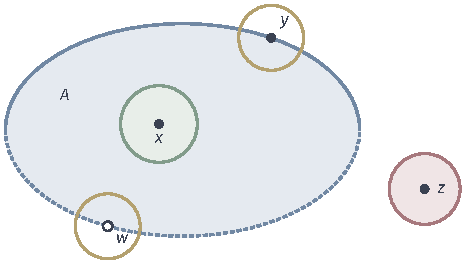
\includegraphics[width=78.807mm]{figures/04-spaces-measures-and-geometry/01-topology-and-metric/tikz/topo-interior-closure/figure.pdf}
  \caption{点与子集的三种关系。$A$是椭圆区域，实线部分的边界属于$A$，虚线部分不属于$A$。$x$有落在$A$内的邻域（绿色），是内点；$z$有与$A$不交的邻域（红色），不在闭包中；$y$与$w$的每个邻域（黄色）都既含$A$的点又含$A$外的点，二者都是边界点，其中$y\in A$，$w\notin A$。}
  \label{fig:topo-interior-closure}
\end{BookInlineFigure}

\paragraph{内部}
点$x$称为$A$的\term{内点}（interior point），如果$A$是$x$的邻域，即有开集$U$满足$x\in U\subseteq A$。$A$的全体内点组成$A$的\term{内部}（interior），记作$\operatorname{int}A$。

把每个内点的这种$U$合起来，得到$\operatorname{int}A$等于含于$A$的所有开集之并，因而它是含于$A$的最大开集。由引理~\ref{lem:topo-open-iff-neighborhood}，$A$开当且仅当$\operatorname{int}A=A$。

\paragraph{闭包}
从另一侧看，点$x$可能不在$A$中，却被$A$紧紧挨着：$x$的每个邻域都含有$A$的点。这时把$x$算作$A$能“接近”的点。

\begin{definition}[闭包]
\label{def:topo-closure}
设$A\subseteq X$。若$x$的每个邻域都与$A$相交，称$x$为$A$的\term{闭包点}（closure point）。$A$的全体闭包点组成的集合称为$A$的\term{闭包}（closure），记作$\overline A$。
\end{definition}

每个邻域都含一个开邻域，所以判断闭包点时只需检验开邻域，或者只需检验某个邻域基的成员。若$x\in A$，则$x$的每个邻域都含$x$，因而与$A$相交，所以$A\subseteq\overline A$。闭包也有一个与内部对称的刻画。

\begin{theorem}[闭包是最小闭超集]
\label{thm:topo-closure-smallest-closed}
对任意$A\subseteq X$，$\overline A$等于所有包含$A$的闭集之交。因此$\overline A$是闭集，并且是包含$A$的最小闭集；$A$闭当且仅当$\overline A=A$。
\end{theorem}
\begin{proof}
记$C$为包含$A$的所有闭集之交。若$x\notin\overline A$，则$x$有开邻域$U$与$A$不交。$X\setminus U$是包含$A$的闭集且不含$x$，所以$x\notin C$。这说明$C\subseteq\overline A$。

反过来，若$x\notin C$，则存在包含$A$的闭集$F$使$x\notin F$。$X\setminus F$是$x$的开邻域，它与$F$不交，因而与$A$不交，$x$不是闭包点。这说明$\overline A\subseteq C$。

闭集之交是闭集，所以$\overline A$闭。其余结论由“最小闭集”直接得到：$A$闭时$A$自己就是包含$A$的最小闭集。
\end{proof}

内部与闭包通过补集相互转换：$x$不是$A$的闭包点，恰好是说$x$有一个开邻域含于$X\setminus A$，即$x$是$X\setminus A$的内点。所以
\begin{equation}
 X\setminus\overline A=\operatorname{int}(X\setminus A).
 \label{eq:topo-closure-interior-complement}
\end{equation}

\paragraph{边界}
闭包与内部之差是那些既能接近$A$、又不被$A$围住的点。称
\begin{equation}
 \partial A=\overline A\setminus\operatorname{int}A
 \label{eq:topo-boundary}
\end{equation}
为$A$的\term{边界}（boundary）。由式~\eqref{eq:topo-closure-interior-complement}，$x\in\partial A$当且仅当$x$的每个邻域都既含$A$的点、又含$X\setminus A$的点。这个判据对$A$与$X\setminus A$对称，所以$\partial A=\partial(X\setminus A)$。

\begin{example}[同一集合在不同拓扑下]
\label{ex:topo-interior-closure-examples}
在$\mathbb R$的通常拓扑下取$A=[0,1)$。$(0,1)$中每点有含于$A$的小区间，$0$没有，所以$\operatorname{int}A=(0,1)$。$1$的每个邻域都含$A$中靠近$1$的点，$[0,1]$外的点有与$A$不交的邻域，所以$\overline A=[0,1]$。由式~\eqref{eq:topo-boundary}，$\partial A=\{0,1\}$。

有理数集$\mathbb Q$的内部为空，因为每个区间都含无理数。它的闭包是$\mathbb R$（见下一小节），所以$\partial\mathbb Q=\mathbb R$。

把$\mathbb R$换成离散拓扑，$A=[0,1)$既开又闭，于是
\[
 \operatorname{int}A=\overline A=A,\qquad\partial A=\varnothing.
\]

换成平凡拓扑，唯一含于$A$的开集是空集，唯一的非空开集$\mathbb R$与$A$相交，所以
\[
 \operatorname{int}A=\varnothing,\qquad\overline A=\mathbb R,\qquad\partial A=\mathbb R.
\]
\end{example}

表~\ref{tab:topo-three-topologies}把结果并排列出。同一个集合在三种拓扑下得到三组完全不同的答案，内部、闭包与边界描述的是集合在某个拓扑中的位置。

\begin{BookInlineTable}
  \centering
  \begin{tabular}{@{}llll@{}}
    \toprule
    $\mathbb R$上的拓扑 & $\operatorname{int}A$ & $\overline A$ & $\partial A$\\
    \midrule
    通常拓扑 & $(0,1)$ & $[0,1]$ & $\{0,1\}$\\
    离散拓扑 & $[0,1)$ & $[0,1)$ & $\varnothing$\\
    平凡拓扑 & $\varnothing$ & $\mathbb R$ & $\mathbb R$\\
    \bottomrule
  \end{tabular}
  \caption{集合$A=[0,1)$在三种拓扑下的内部、闭包与边界。}
  \label{tab:topo-three-topologies}
\end{BookInlineTable}

有限空间上可以完整地算一遍。取图~\ref{fig:topo-finite-topologies}(b)的拓扑，它的开集是$\varnothing,\{a\},\{a,b\},X$，取补集得到闭集
\[
 X,\quad\{b,c\},\quad\{c\},\quad\varnothing.
\]

设$A=\{b\}$。含于$A$的开集只有$\varnothing$，所以$\operatorname{int}A=\varnothing$。包含$A$的闭集是$\{b,c\}$与$X$，它们的交是$\{b,c\}$，由定理~\ref{thm:topo-closure-smallest-closed}得到
\[
 \overline A=\{b,c\},\qquad\partial A=\{b,c\}.
\]
点$c$也在闭包里，因为$c$唯一的开邻域$X$含有$b$。

在有距离的空间里，闭包点还能用“到$A$的距离为零”来刻画，这一判据依赖度量，放在第~\ref{chap:metric-spaces}章建立。

\subsection{稠密集}
\label{sec:topo-dense-sets}

每个实数都能被有理数任意接近，用闭包的语言，这就是说$\mathbb Q$的闭包是整个$\mathbb R$。把这一性质抽象出来，就是稠密。

\begin{definition}[稠密集]
\label{def:topo-dense}
若$D\subseteq X$满足$\overline D=X$，称$D$在$X$中\term{稠密}（dense）。
\end{definition}

由闭包的定义，$\overline D=X$意味着每个点的每个邻域都与$D$相交。每个非空开集都是它每个点的邻域，所以这又可以写成只涉及开集的判据。

\begin{theorem}[稠密的开集判据]
\label{thm:topo-dense-open-criterion}
$D$在$X$中稠密，当且仅当$X$的每个非空开集都与$D$相交。
\end{theorem}
\begin{proof}
设$D$稠密，$U$是非空开集，取$x\in U$。$U$是$x$的邻域，而$x\in\overline D$，所以$U\cap D\neq\varnothing$。

反过来，设每个非空开集都与$D$相交。任取$x\in X$及其邻域$N$，$N$含某个开集$U\ni x$。$U$非空，故与$D$相交，于是$N$也与$D$相交，$x\in\overline D$。
\end{proof}

\begin{example}[有理数与无理数都稠密]
\label{ex:topo-rationals-irrationals-dense}
由定理~\ref{thm:topo-dense-open-criterion}，只需证明每个开区间$(a,b)$（$a<b$）都含有理数和无理数。

由实数的Archimedes性质（由确界原理推出，可参考\BookChapterRef{chap:real-complex-functions}{卷一第4章“实数、复数与函数”}），可取正整数$n$使$1/n<b-a$，再取最小的整数$m$使$m/n>a$。由$m$的最小性，$(m-1)/n\leq a$，所以
\[
 a<\frac mn\leq a+\frac1n<b.
\]

用数字走一遍。设$(a,b)=(0.3,0.31)$，长度为$0.01$，取$n=101$。$30/101\approx0.2970$还小于$0.3$，所以$m=31$，得到
\[
 \frac{31}{101}\approx0.3069\in(0.3,0.31).
\]

对无理数，把同样的论证用于区间$(a-\sqrt2,b-\sqrt2)$，得到其中的有理数$q$，则$q+\sqrt2\in(a,b)$。$q+\sqrt2$是无理数，否则$\sqrt2=(q+\sqrt2)-q$会是有理数。所以$\mathbb Q$与$\mathbb R\setminus\mathbb Q$都在$\mathbb R$中稠密，而它们互不相交。
\end{example}

稠密并不要求子集占据大部分空间。$\mathbb Q$与无理数集都稠密，却彼此不交；第~\ref{chap:measure}章还会看到，$\mathbb Q$的长度为零。稠密只说明子集能接近空间中的每一点，并没有覆盖它们。

\paragraph{为什么不用点列定义稠密}
在$\mathbb R$中，$D$稠密等价于每个实数都是$D$中某个点列的极限。一般拓扑空间中，邻域可能多到无法用可数个依次缩小的集合代表，点列这时走不到闭包中的所有点。第~\ref{sec:topo-convergence}节将给出这样的空间，所以闭包与稠密性都以邻域定义，点列判据只在附加条件下成立。


\section{点列收敛}
\label{sec:topo-convergence}

实数列$x_n\to x$的定义是：对每个$\varepsilon>0$，存在$N$，使$n\geq N$时$\lvert x_n-x\rvert<\varepsilon$。条件$\lvert x_n-x\rvert<\varepsilon$就是$x_n\in(x-\varepsilon,x+\varepsilon)$，所以这句话等于说：对$x$的邻域基中每个区间，点列最终停在其中。把邻域基换成全部邻域，就得到不需要距离的收敛定义。

\begin{definition}[点列收敛]
\label{def:topo-sequence-convergence}
设$X$是拓扑空间，$(x_n)_{n\geq1}$是$X$中的点列，$x\in X$。若对$x$的每个邻域$N$，都存在$n_0$使$n\geq n_0$时$x_n\in N$，就称$(x_n)$\term{收敛}（converge）到$x$，记作$x_n\to x$，并称$x$为点列的一个\term{极限}（limit）。
\end{definition}

由于$x$的每个邻域都包含邻域基中的成员，只需对某个邻域基的成员检验这个条件。在$\mathbb R$上取邻域基$\{(x-\varepsilon,x+\varepsilon):\varepsilon>0\}$，定义~\ref{def:topo-sequence-convergence}就逐字回到实数列极限的$\varepsilon$-$N$定义，所以通常拓扑下的收敛与卷一的极限完全一致。

\paragraph{拓扑决定哪些点列收敛}
收敛完全由邻域决定，因此随拓扑而变。在离散拓扑中，$\{x\}$是$x$的邻域，$x_n\to x$意味着点列最终恒等于$x$。在平凡拓扑中，$x$的唯一邻域是整个空间，每个点列都收敛到每个点，极限可以不唯一。极限何时唯一，取决于不同点能否用不交的邻域分开，这是第~\ref{sec:topo-separation}小节的问题；在那之前，我们只说“一个极限”，而不说“极限”。

\paragraph{子列与闭集}
实数列的两条基本性质只用到邻域，因此在一般拓扑空间中照样成立：收敛点列的子列收敛到同一个点，闭集不会让其中点列的极限跑到集合外面。

\begin{theorem}[子列与闭包]
\label{thm:topo-subsequence-closure}
设$x_n\to x$。
\begin{enumerate}
  \item 对任意子列$(x_{n_k})$（$n_1<n_2<\cdots$），$x_{n_k}\to x$；
  \item 若所有$x_n$都属于集合$A$，则$x\in\overline A$；特别地，若$A$是闭集，则$x\in A$。
\end{enumerate}
\end{theorem}
\begin{proof}
对$x$的邻域$N$，取$n_0$使$n\geq n_0$时$x_n\in N$。由于$n_k\geq k$，当$k\geq n_0$时$n_k\geq n_0$，于是$x_{n_k}\in N$，第一条成立。

对第二条，$x$的每个邻域$N$都含有某个$x_n$，而$x_n\in A$，所以$N$与$A$相交，$x$是$A$的闭包点。$A$闭时$\overline A=A$。
\end{proof}

\paragraph{点列不能反推闭包}
在$\mathbb R$中，定理~\ref{thm:topo-subsequence-closure}的第二条可以反过来：$\overline A$中的每个点都是$A$中某个点列的极限，这是卷一闭集序列判据的内容。下面的例子说明，在一般拓扑空间中这个逆命题不成立，这也是第~\ref{sec:topo-dense-sets}小节不用点列定义稠密性的原因。

\begin{example}[余可数拓扑]
\label{ex:topo-cocountable}
在$\mathbb R$上规定：$U$为开集当且仅当$U=\varnothing$或$\mathbb R\setminus U$是可数集（有限或可数无限）。可数集的任意交、有限并仍可数，所以这些$U$对任意并和有限交封闭，构成一个拓扑，称为\term{余可数拓扑}（cocountable topology）。它的闭集是$\mathbb R$本身与全部可数集。

先看收敛的点列。设$x_n\to x$，令$C=\{x_n:x_n\neq x\}$，它是可数集，所以$\mathbb R\setminus C$是含$x$的开集。点列最终落在其中，即$n$充分大时$x_n\notin C$，也就是$x_n=x$。所以在这个拓扑中，只有最终恒定的点列才收敛。

再取$A=\mathbb R\setminus\{0\}$。包含$A$的闭集只能是$\mathbb R$，因为可数集不能包含不可数集$A$；于是$\overline A=\mathbb R\ni0$。但$A$中的点列若收敛，最终恒等于某个$A$中的点，极限不可能是$0$。所以$0\in\overline A$，却不是$A$中任何点列的极限。同时，$A$中收敛点列的极限都在$A$内，而$A$不是闭集：“包含点列的所有极限”在这里推不出闭性。
\end{example}

问题出在邻域的数量上。在$\mathbb R$的通常拓扑中，$0$的可数个邻域$(-1/k,1/k)$就能代表所有邻域，从每个中选一点即可造出趋于$0$的点列。余可数拓扑中$0$没有这样的可数邻域基：若$N_1,N_2,\dots$是$0$的邻域，各含开集$U_k\ni0$，则$\bigcup_k(\mathbb R\setminus U_k)$是可数个可数集之并，仍可数，于是可取$y\neq0$属于所有$U_k$；开集$\mathbb R\setminus\{y\}$是$0$的邻域，却不包含任何$N_k$。

第~\ref{sec:topo-countability}小节把“有可数邻域基”定义为第一可数性；在度量空间中这一条件自动成立，闭包与闭集的序列判据在第~\ref{chap:metric-spaces}章证明。


\section{连续映射}
\label{sec:topo-continuous-maps}

前两节研究一个空间内部的子集与点列，本节转向两个空间之间的映射。实函数$f$在$x_0$处连续的含义是：只要输入留在$x_0$附近某个足够小的区间内，输出就留在$f(x_0)$附近指定的区间内。这个要求可以改用开集表达，从而推广到任意拓扑空间。

\subsection{连续性的定义}
\label{sec:topo-continuity-definition}

先看$\varepsilon$-$\delta$定义在说什么。给定连续的$f:\mathbb R\to\mathbb R$及开集$V\subseteq\mathbb R$，设$f(x_0)\in V$，取$\varepsilon$使$(f(x_0)-\varepsilon,f(x_0)+\varepsilon)\subseteq V$。连续性给出$\delta>0$，使
\[
 (x_0-\delta,x_0+\delta)\subseteq f^{-1}(V).
\]
这对$f^{-1}(V)$的每个点成立，所以$f^{-1}(V)$是开集。逐点的“输入附近映入输出附近”就这样变成了一句关于原像的话。

图~\ref{fig:topo-preimage}(a)取$f(x)=x^2$，$V=(1,4)$，解$1<x^2<4$得
\[
 f^{-1}(V)=(-2,-1)\cup(1,2),
\]
这是开集。在点$x_0=3/2$处，$(1,2)$就是一个可用的区间，对应$\delta=1/2$。

图~\ref{fig:topo-preimage}(b)是有跳跃的函数，$x<1$时$f(x)=x$，$x\geq1$时$f(x)=x+1$。取$V=(3/2,5/2)$，$x<1$的部分取值小于$1$，不进入$V$；$x\geq1$的部分要求$x+1<5/2$。于是
\[
 f^{-1}(V)=[1,3/2),
\]
它含左端点而在那里没有余地，不是开集。跳跃恰好表现为某个开集的原像不开。

\begin{BookInlineFigure}
  \centering
  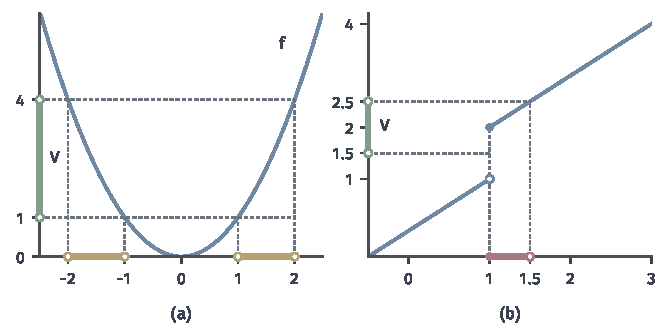
\includegraphics[width=112mm]{figures/04-spaces-measures-and-geometry/01-topology-and-metric/matplotlib/topo-preimage/figure.pdf}
  \caption{开集的原像。绿色是纵轴上的开区间$V$。(a)$f(x)=x^2$，$V=(1,4)$的原像是横轴上的$(-2,-1)\cup(1,2)$（黄色），仍是开集。(b)$f$在$x=1$处跳跃，$V=(3/2,5/2)$的原像是$[1,3/2)$（红色），含端点$1$，不是开集。}
  \label{fig:topo-preimage}
\end{BookInlineFigure}

\begin{definition}[连续映射]
\label{def:topo-continuous-map}
设$X,Y$是拓扑空间。映射$f:X\to Y$称为\term{连续映射}（continuous map），如果对$Y$的每个开集$V$，下面的原像都是$X$的开集：
\begin{equation}
 f^{-1}(V)=\{x\in X:f(x)\in V\}.
 \label{eq:topo-preimage}
\end{equation}
\end{definition}

定义用原像，是因为原像与集合运算相容：
\[
\begin{gathered}
 f^{-1}\Bigl(\bigcup_iV_i\Bigr)=\bigcup_if^{-1}(V_i),\qquad
 f^{-1}\Bigl(\bigcap_iV_i\Bigr)=\bigcap_if^{-1}(V_i),\\
 f^{-1}(Y\setminus V)=X\setminus f^{-1}(V).
\end{gathered}
\]
这些等式可参考\BookChapterRef{chap:sets-relations-maps}{卷一第1章“集合、关系与映射”}。由第一个等式，若$\mathcal B$是$Y$的拓扑基，只需检验每个$B\in\mathcal B$的原像为开集，因为任意开集都是基本开集之并。

\paragraph{等价判据}
定义~\ref{def:topo-continuous-map}是整体的说法。处理具体映射时，有时逐点检验更方便，有时检验闭集更方便。

\begin{theorem}[连续性的等价刻画]
\label{thm:topo-continuity-equivalent}
对映射$f:X\to Y$，下列条件等价：
\begin{enumerate}
  \item $f$连续；
  \item 对每个$x\in X$及$f(x)$的每个邻域$V$，存在$x$的邻域$U$使$f(U)\subseteq V$；
  \item 对$Y$的每个闭集$F$，$f^{-1}(F)$是$X$的闭集。
\end{enumerate}
\end{theorem}
\begin{proof}
1推出2。$V$含开集$V'\ni f(x)$，$U=f^{-1}(V')$是含$x$的开集，并且$f(U)\subseteq V'\subseteq V$。

2推出1。设$V$开，$x\in f^{-1}(V)$。$V$是$f(x)$的邻域，取$x$的邻域$U$使$f(U)\subseteq V$，则$U\subseteq f^{-1}(V)$。所以$f^{-1}(V)$是它每个点的邻域，由引理~\ref{lem:topo-open-iff-neighborhood}是开集。

1与3的等价来自等式$f^{-1}(Y\setminus F)=X\setminus f^{-1}(F)$：闭集的补集是开集，原像的补集是补集的原像。
\end{proof}

条件2在$X=Y=\mathbb R$时取邻域基$(x-\delta,x+\delta)$与$(f(x)-\varepsilon,f(x)+\varepsilon)$，就是$\varepsilon$-$\delta$定义，所以通常拓扑下的连续与卷一的连续一致。常值映射总是连续的，因为任何集合的原像只能是$\varnothing$或$X$。

\begin{example}[连续性依赖两边的拓扑]
\label{ex:topo-continuity-depends-topology}
考虑恒等映射$\operatorname{id}:\mathbb R\to\mathbb R$。若定义域取离散拓扑，则无论值域取什么拓扑，它都连续，因为定义域的每个子集都开。

若定义域取通常拓扑、值域取离散拓扑，则$\{0\}$在值域中开，原像$\{0\}$在定义域中不开，恒等映射不连续。同一个集合映射，连续与否由两边的开集族共同决定。
\end{example}

\paragraph{复合与点列}
连续映射的复合仍然连续。设$f:X\to Y$与$g:Y\to Z$连续，$W$是$Z$的开集，则
\[
 (g\circ f)^{-1}(W)=f^{-1}\bigl(g^{-1}(W)\bigr).
\]
先由$g$连续得到$g^{-1}(W)$开，再由$f$连续得到它的原像开。连续映射也保持已有的点列极限。

\begin{theorem}[连续映射保持极限]
\label{thm:topo-continuous-preserves-limits}
设$f:X\to Y$连续，$X$中的点列$x_n\to x$，则$f(x_n)\to f(x)$。
\end{theorem}
\begin{proof}
设$V$是$f(x)$的邻域。由定理~\ref{thm:topo-continuity-equivalent}，有$x$的邻域$U$使$f(U)\subseteq V$。由$x_n\to x$，$n$充分大时$x_n\in U$，于是$f(x_n)\in V$。
\end{proof}

反过来，“保持所有收敛点列的极限”能否推出连续，取决于点列能否探测定义域的拓扑。在余可数拓扑（例~\ref{ex:topo-cocountable}）中只有最终恒定的点列收敛，所以从这个空间出发的任何映射都保持极限。

然而从余可数拓扑的$\mathbb R$到通常拓扑的$\mathbb R$的恒等映射并不连续：开集$(0,1)$的补集不可数，原像$(0,1)$不是余可数拓扑的开集。在度量空间中，序列判据与连续性等价，这在第~\ref{chap:metric-space-maps}章证明。

\paragraph{原像与像}
连续性约束的是原像，对像没有直接约束。连续映射$f(x)=x^2$把开区间$(-1,1)$映成$[0,1)$，见图~\ref{fig:topo-image-openness}(a)，它不是开集。连续映射$g(x)=\arctan x$把闭集$\mathbb R$映成$(-\pi/2,\pi/2)$，它不是闭集。

像对集合运算的行为也不如原像整齐：像与并相容，但$f(A\cap B)$一般只包含于$f(A)\cap f(B)$。取$f(x)=x^2$，$A=\{-1\}$，$B=\{1\}$，则
\[
 f(A\cap B)=\varnothing,\qquad f(A)\cap f(B)=\{1\}.
\]

\subsection{开映射}
\label{sec:topo-open-maps}

上一小节的例子提出另一个问题：哪些映射把开集映成开集？这个条件与连续性平行，方向却相反。

\begin{definition}[开映射]
\label{def:topo-open-map}
映射$f:X\to Y$称为\term{开映射}（open map），如果对$X$的每个开集$U$，像$f(U)$是$Y$的开集。
\end{definition}

由于$f(\bigcup_iU_i)=\bigcup_if(U_i)$，验证开映射只需对定义域的某个拓扑基检验。

两个条件互不蕴含。常值映射$f(x)=c$连续，但$f((0,1))=\{c\}$不是开集，所以连续不保证开映射。反过来，从通常拓扑到离散拓扑的恒等映射（例~\ref{ex:topo-continuity-depends-topology}）把每个集合映成离散拓扑中的开集，是开映射，却不连续。

开映射的典型例子是平面到坐标轴的投影$p(x_1,x_2)=x_1$。开矩形$(a_1,b_1)\times(a_2,b_2)$的像是$(a_1,b_1)$，而开矩形构成拓扑基，所以$p$是开映射，见图~\ref{fig:topo-image-openness}(b)。

开映射也不必把闭集映成闭集。双曲线$\{(x_1,x_2):x_1x_2=1\}$是连续函数$x_1x_2$在闭集$\{1\}$上的原像，因而闭，它在$p$下的像却是$\mathbb R\setminus\{0\}$，见图~\ref{fig:topo-image-openness}(c)。这个像不含$0$，而$0$是它的闭包点，所以不闭。

\begin{BookInlineFigure}
  \centering
  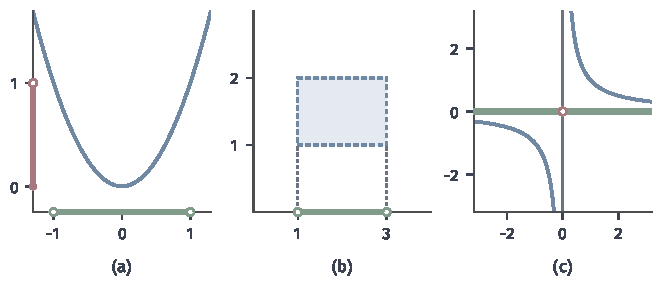
\includegraphics[width=112mm]{figures/04-spaces-measures-and-geometry/01-topology-and-metric/matplotlib/topo-image-openness/figure.pdf}
  \caption{像的开闭性。(a)$f(x)=x^2$把绿色开区间$(-1,1)$映成纵轴上的$[0,1)$（红色），连续而不开。(b)投影把开矩形$(1,3)\times(1,2)$映成开区间$(1,3)$。(c)闭集$x_1x_2=1$在投影下的像是绿色的$\mathbb R\setminus\{0\}$，缺少原点，不闭。}
  \label{fig:topo-image-openness}
\end{BookInlineFigure}

\subsection{同胚}
\label{sec:topo-homeomorphisms}

两个拓扑空间什么时候应当看作“相同”？线性代数中，可逆线性映射把一边的线性结构原样搬到另一边，于是两个同构的线性空间不必区分。拓扑中的对应角色是：一个双射把一边的开集恰好对应到另一边的开集。这时一切只用开集表述的概念（邻域、闭包、收敛、连续）都会被这个双射原样搬过去。

\begin{definition}[同胚]
\label{def:topo-homeomorphism}
双射$f:X\to Y$称为\term{同胚}（homeomorphism），如果$f$与逆映射$f^{-1}$都连续。存在同胚时，称$X$与$Y$同胚，记作$X\cong Y$。
\end{definition}

$f$连续说明$Y$的开集对应到$X$的开集。$f^{-1}$连续说明$X$的开集$U$的像$f(U)=(f^{-1})^{-1}(U)$是$Y$的开集。所以同胚在两边的开集族之间建立了一一对应，$x$的邻域也恰好对应到$f(x)$的邻域。

\begin{theorem}[连续双射成为同胚的条件]
\label{thm:topo-homeomorphism-open}
设$f:X\to Y$是连续双射。$f$是同胚，当且仅当$f$是开映射。
\end{theorem}
\begin{proof}
对$X$的开集$U$，$f$是双射，所以
\[
 (f^{-1})^{-1}(U)=\{y:f^{-1}(y)\in U\}=f(U).
\]
于是“$f^{-1}$连续”逐字等于“$f$把每个开集映成开集”。
\end{proof}

连续双射未必是同胚。例~\ref{ex:topo-continuity-depends-topology}中从离散拓扑到通常拓扑的恒等映射是连续双射，但不是开映射，因为$\{0\}$的像不开。第~\ref{sec:topo-subspaces}小节还会给出一个更直观的例子：把半开区间绕成圆周的映射。

\paragraph{同胚不保持长度}
同胚只要求开集对应，不要求保持距离、长度或有界性。仿射映射$x\mapsto a+(b-a)x$是$(0,1)$到$(a,b)$的同胚，它把长度伸缩了$b-a$倍。更进一步，映射
\begin{equation}
 h:(-1,1)\to\mathbb R,\qquad h(x)=\frac{x}{1-\lvert x\rvert}
 \label{eq:topo-interval-line-homeomorphism}
\end{equation}
把有界区间变成整条实轴。

它的逆映射是$h^{-1}(y)=y/(1+\lvert y\rvert)$。验证一下，设$y\geq0$，$x=y/(1+y)$，则$1-\lvert x\rvert=1/(1+y)$，于是
\[
 h(x)=\frac{y/(1+y)}{1/(1+y)}=y.
\]
$y<0$时由$h$是奇函数得到同样的结论。$h$与$h^{-1}$都由连续函数作除法得到，分母不为零，所以都连续。

在具体的点上，$h(1/2)=1$，$h(3/4)=3$，图~\ref{fig:topo-homeomorphism}(a)标出了这些点。输入越靠近$\pm1$，输出越大，距离被任意放大，开集的对应却没有被破坏。

\begin{BookInlineFigure}
  \centering
  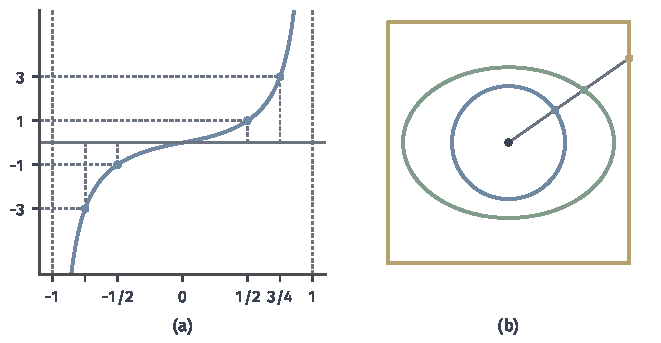
\includegraphics[width=112mm]{figures/04-spaces-measures-and-geometry/01-topology-and-metric/matplotlib/topo-homeomorphism/figure.pdf}
  \caption{同胚不保持度量性质。(a)$h(x)=x/(1-\lvert x\rvert)$把$(-1,1)$连续地拉成整条实轴，图中标出了$\pm1/2$与$\pm3/4$的函数值$\pm1$与$\pm3$。(b)从中心出发的射线与圆周、椭圆、正方形边界各交一点，沿射线移动这些交点就得到三条曲线之间的同胚。}
  \label{fig:topo-homeomorphism}
\end{BookInlineFigure}

有界性、长度都不是拓扑性质。拓扑性质指同胚保持的性质，例如本章后面的连通性与紧性。

同样，平面上的单位圆周与正方形边界同胚，这里的正方形边界是
\[
 \{\bm y:\max(\lvert y_1\rvert,\lvert y_2\rvert)=1\}.
\]
从原点出发的每条射线与两条曲线各交于一点，沿射线移动的映射是
\[
 F(\bm x)=\frac{\bm x}{\max(\lvert x_1\rvert,\lvert x_2\rvert)},\qquad
 F^{-1}(\bm y)=\frac{\bm y}{\sqrt{y_1^2+y_2^2}}.
\]

取$\bm x=(3/5,4/5)$，除以$4/5$得$F(\bm x)=(3/4,1)$；再除以其长度$5/4$，回到$(3/5,4/5)$。图~\ref{fig:topo-homeomorphism}(b)还画了椭圆，同样的射线也给出它与另外两条曲线的对应。三者周长和弯曲程度各不相同，拓扑只记录它们首尾相接成一圈的结构。要严格核对这类平面子集上的开集，需要下一节的子空间拓扑。


\section{空间的构造}
\label{sec:topo-constructions}

很多空间是从已有空间造出来的：圆周是平面的一部分，随时间运动的位置取值于“空间乘以时间”，圆周也可以由线段把两端粘合得到。这三种构造各有一个自然的映射，即包含映射、坐标投影和商映射。新空间的开集，就按“使这个映射连续”来规定，这条规则同时给出了判断映入或映出新空间的映射何时连续的方法。

\subsection{子空间}
\label{sec:topo-subspaces}

研究圆周$S^1=\{(x_1,x_2)\in\mathbb R^2:x_1^2+x_2^2=1\}$时，我们希望沿用平面的“附近”：圆周上一点附近，就是平面上这点附近与圆周的公共部分。

\begin{definition}[子空间拓扑]
\label{def:topo-subspace}
设$(X,\mathcal T)$是拓扑空间，$A\subseteq X$。下面的族是$A$上的拓扑，称为\term{子空间拓扑}（subspace topology）：
\begin{equation}
 \mathcal T_A=\{U\cap A:U\in\mathcal T\}.
 \label{eq:topo-subspace}
\end{equation}
称$(A,\mathcal T_A)$为$X$的子空间，$\mathcal T_A$的成员称为在$A$中\term{相对开}（relatively open）的集合。
\end{definition}

$\mathcal T_A$确实是拓扑：$\varnothing\cap A$与$X\cap A$分别给出$\varnothing$与$A$，并且
\[
 \bigcup_i(U_i\cap A)=\Bigl(\bigcup_iU_i\Bigr)\cap A,\qquad
 (U\cap A)\cap(V\cap A)=(U\cap V)\cap A.
\]

对补集取交同样可得：$A$中的相对闭集恰是形如$F\cap A$的集合，$F$为$X$的闭集。若$\mathcal B$是$X$的拓扑基，则$\{B\cap A:B\in\mathcal B\}$是子空间拓扑的基。

\paragraph{相对开与在环境中开}
相对开放比在环境中开放的要求低。取$X=\mathbb R$，$A=[0,1]$。如图~\ref{fig:topo-subspace-wrap}(a)，集合
\[
 [0,1/2)=(-1,1/2)\cap A
\]
在$A$中相对开，在$\mathbb R$中却不开。$A$本身作为子空间是全空间，因而在$A$中既开又闭，在$\mathbb R$中它只是闭集。

端点处的邻域只需单侧：$0$在$A$中的邻域基可以取$[0,1/k)$，$k\geq1$。单点集$\{0\}$在$A$中仍不开，因为每个相对开的含$0$集合都含有某个$[0,\varepsilon)$。

当$A$本身在$X$中开时，相对开集就是含于$A$的$X$的开集，因为两个开集的交仍开。上面的差别只出现在非开的子集上。描述子集的开闭性时，因此必须说明环境：“在$A$中开”与“在$X$中开”是两回事。

\paragraph{映入子空间的映射}
包含映射$\iota:A\to X$，$\iota(a)=a$，是连续的，因为$\iota^{-1}(U)=U\cap A$。子空间拓扑恰好使这一点成立：它是$A$上使$\iota$连续的最粗拓扑。因此，连续映射$f:X\to Y$限制到子空间上仍连续，因为$f|_A=f\circ\iota$。

\begin{lemma}[映入子空间的映射]
\label{lem:topo-map-into-subspace}
设$A\subseteq Y$为子空间，$g:Z\to A$。则$g$连续，当且仅当$\iota\circ g:Z\to Y$连续。
\end{lemma}
\begin{proof}
必要性是复合的连续性。充分性：$A$的每个开集形如$V\cap A$，$V$为$Y$的开集，而
\[
 g^{-1}(V\cap A)=(\iota\circ g)^{-1}(V)
\]
是开集。
\end{proof}

判断一个映入圆周的映射是否连续，只需把它看成映入平面的映射，逐坐标检验。例如$p(t)=(\cos2\pi t,\sin2\pi t)$作为$\mathbb R\to\mathbb R^2$连续（下一小节说明为什么可以逐坐标判断），因而作为$\mathbb R\to S^1$也连续。

\begin{example}[把半开区间绕成圆周]
\label{ex:topo-interval-to-circle}
限制$p$得到$p:[0,1)\to S^1$，其中$[0,1)$取$\mathbb R$的子空间拓扑。$p$是连续双射：圆周上的每个点恰对应$[0,1)$中的一个参数。但它不是同胚。

集合$[0,1/2)$在$[0,1)$中相对开，它的像是从$(1,0)$出发、沿逆时针走到$(-1,0)$之前的半圆弧，含端点$(1,0)$而不含$(-1,0)$。

这条弧在$S^1$中不是相对开的：$(1,0)$在$S^1$中的每个邻域都含有某个$p(t)$，其中$t$接近$1$，这些点位于$x_2<0$的一侧，不在弧上。所以$p$不是开映射，由定理~\ref{thm:topo-homeomorphism-open}，它不是同胚。
\end{example}

图~\ref{fig:topo-subspace-wrap}(b)显示了失败的原因：$[0,1)$在$0$处只有右侧的邻域，而圆周在$(1,0)$处两侧都有邻域。$p$把点一一对应，却没有对应它们的附近。

\begin{BookInlineFigure}
  \centering
  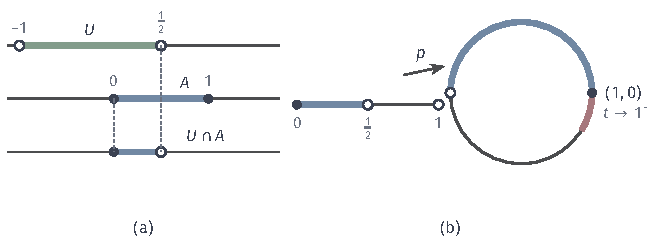
\includegraphics[width=111.774mm]{figures/04-spaces-measures-and-geometry/01-topology-and-metric/tikz/topo-subspace-wrap/figure.pdf}
  \caption{子空间中的相对开集。(a)绿色的$U=(-1,1/2)$在$\mathbb R$中开，与蓝色的$A=[0,1]$相交得到$[0,1/2)$，它在$A$中相对开，在$\mathbb R$中不开。(b)$p$把$[0,1/2)$（蓝色）绕成上半圆弧，弧含$(1,0)$；$(1,0)$下方的点（红色）来自$t$接近$1$的参数，不在弧上，所以弧不相对开。}
  \label{fig:topo-subspace-wrap}
\end{BookInlineFigure}

\subsection{有限乘积}
\label{sec:topo-finite-products}

描述平面上的位置需要两个实坐标，描述一个随时间变化的位置需要“空间中的点”与“时刻”两个分量。这类成对的数据取值于乘积集合$X\times Y$，我们需要在其上规定开集，使“两个分量都在各自的附近”成为乘积中的附近。

\begin{definition}[乘积拓扑]
\label{def:topo-product}
设$X,Y$是拓扑空间。下面的族生成的拓扑称为$X\times Y$上的\term{乘积拓扑}（product topology）：
\begin{equation}
 \mathcal B=\{U\times V:U\text{在}X\text{中开},\ V\text{在}Y\text{中开}\}.
 \label{eq:topo-product-basis}
\end{equation}
有限个空间$X_1\times\cdots\times X_n$的乘积拓扑同样由$U_1\times\cdots\times U_n$生成。
\end{definition}

$\mathcal B$满足定理~\ref{thm:topo-basis-criterion}的条件：$X\times Y$本身属于$\mathcal B$，并且
\[
 (U_1\times V_1)\cap(U_2\times V_2)=(U_1\cap U_2)\times(V_1\cap V_2)
\]
仍属于$\mathcal B$。

乘积拓扑的开集一般不是“开集乘开集”，而是这些开矩形的并，例如$\mathbb R^2$中的开圆盘。取$X=Y=\mathbb R$，这正是例~\ref{ex:topo-intervals-rectangles}中由开矩形生成的通常拓扑。若$X,Y$分别有拓扑基$\mathcal B_X,\mathcal B_Y$，则$\{B\times B':B\in\mathcal B_X,\ B'\in\mathcal B_Y\}$也是乘积拓扑的基。

\paragraph{投影与分量}
坐标投影$\pi_X(x,y)=x$与$\pi_Y(x,y)=y$是连续的：$\pi_X^{-1}(U)=U\times Y$是基本开集。它们也是开映射，因为基本开集$U\times V$（$V\neq\varnothing$）的像是开集$U$。

乘积拓扑是使两个投影都连续的最粗拓扑：若投影连续，$U\times Y$与$X\times V$必须开，它们的交$U\times V$也就必须开，图~\ref{fig:topo-product-neighborhood}(a)画的就是这个交。这一性质给出下面的判据。

\begin{theorem}[映入乘积的映射]
\label{thm:topo-map-into-product}
设$f:Z\to X\times Y$，写作$f(z)=(f_1(z),f_2(z))$，其中$f_1=\pi_X\circ f$，$f_2=\pi_Y\circ f$。则$f$连续，当且仅当$f_1$与$f_2$都连续。
\end{theorem}
\begin{proof}
若$f$连续，$f_1,f_2$是连续映射的复合，因而连续。

反过来，设$f_1,f_2$连续。对基本开集$U\times V$，有
\[
 f^{-1}(U\times V)=f_1^{-1}(U)\cap f_2^{-1}(V),
\]
这是两个开集的交，因而开。任意开集是基本开集之并，其原像是这些原像之并，所以$f$连续。
\end{proof}

由此，$\mathbb R^n$中的映射可以逐坐标判断连续性，上一小节的$p(t)=(\cos2\pi t,\sin2\pi t)$连续，正是因为两个分量都是连续实函数。这个判据只对映入乘积的映射成立。从乘积出发的映射，即使对每个分量单独连续，也未必整体连续：
\[
 f(x_1,x_2)=\frac{x_1x_2}{x_1^2+x_2^2}\quad(\text{原点处补定义为}0)
\]
在固定任一分量时对另一分量连续，沿对角线$x_1=x_2\neq0$却恒为$1/2$，所以在原点不连续。

\paragraph{空间与区间的乘积}
设$X$是拓扑空间，$I=[0,1]$取$\mathbb R$的子空间拓扑。乘积$X\times I$的点$(x,t)$可以理解为“时刻$t$时位于$x$”。一个连续映射$H:X\times I\to Y$同时记录了一族映射$H_t=H(\cdot,t):X\to Y$，$t\in I$。

乘积拓扑保证这族映射随$t$连续变化：如图~\ref{fig:topo-product-neighborhood}(b)，$(x,t)$的邻域含形如$U\times(t-\delta,t+\delta)$的基本开集（在$I$的端点处只取单侧），所以$x$附近、$t$附近的输入都映到$H(x,t)$附近。每个$H_t$连续，是因为它是$H$与连续映射$x\mapsto(x,t)$的复合。

\begin{BookInlineFigure}
  \centering
  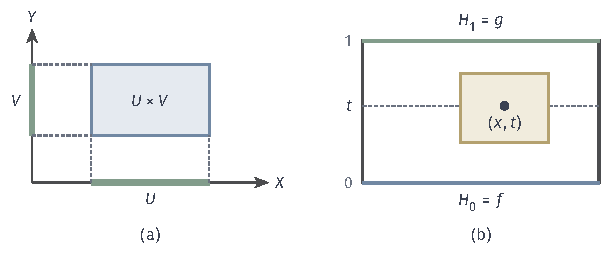
\includegraphics[width=102.404mm]{figures/04-spaces-measures-and-geometry/01-topology-and-metric/tikz/topo-product-neighborhood/figure.pdf}
  \caption{乘积拓扑的基本开集。(a)$U\times V$是投影下$U$与$V$的原像之交。(b)$X\times I$中$H_0=f$在底边，$H_1=g$在顶边，虚线是某一时刻的$H_t$；黄色方块是$(x,t)$的基本开邻域，同时限制空间位置与时刻。}
  \label{fig:topo-product-neighborhood}
\end{BookInlineFigure}

例如，对两个连续映射$f,g:X\to\mathbb R^n$，令
\[
 H(x,t)=(1-t)f(x)+tg(x).
\]
由定理~\ref{thm:topo-map-into-product}，$(x,t)\mapsto(f(x),g(x),t)$连续，$H$的每个坐标是这些分量经实数加法、乘法得到的，加法与乘法作为$\mathbb R^2\to\mathbb R$的映射连续，所以$H$连续。这时$H_0=f$，$H_1=g$，$H$把$f$逐渐变成$g$。

这种从一个映射连续变形到另一个映射的对象称为同伦，它是第~\ref{chap:homology}章的出发点，乘积$X\times I$正是它的定义域。

\subsection{商空间}
\label{sec:topo-quotients}

把一张纸条的两端粘起来，得到一个圈；把正方形的对边分别粘合，得到一个环面。这类构造把原空间中若干点看作同一点，然后问：粘合后的集合上，哪些子集应当算开集？

\paragraph{等价类与投影}
用等价关系$\sim$描述“看作同一点”：$x\sim y$表示$x$与$y$被识别。设$X/{\sim}$为全体等价类$[x]=\{y\in X:y\sim x\}$组成的集合，$q:X\to X/{\sim}$，$q(x)=[x]$，为把每点送到所在类的投影。我们希望$q$连续，而且在这一前提下尽可能多地保留开集。

\begin{definition}[商拓扑]
\label{def:topo-quotient}
设$X$是拓扑空间，$\sim$是$X$上的等价关系。规定$V\subseteq X/{\sim}$为开集，当且仅当$q^{-1}(V)$是$X$的开集。这样得到的拓扑称为\term{商拓扑}（quotient topology），$X/{\sim}$配上商拓扑称为\term{商空间}（quotient space），$q$称为\term{商映射}（quotient map）。
\end{definition}

原像与并、交相容，所以这个族满足拓扑的三条规则。按定义$q$连续，并且商拓扑是使$q$连续的最细拓扑：若$X/{\sim}$上的某个拓扑使$q$连续，它的每个开集$V$都满足$q^{-1}(V)$开，从而属于商拓扑。

子空间、乘积用“最粗”，商空间用“最细”，方向相反的原因在于新拓扑所在的一侧。包含映射与投影的新拓扑在定义域一侧，开集越多映射越容易连续，连续性只给出开集的下限，所以取满足下限的最粗者。商映射的新拓扑在值域一侧，开集越少映射越容易连续，连续性只给出开集的上限，所以取满足上限的最细者。

$q^{-1}(V)$是若干完整等价类之并，所以商空间的开集恰好对应$X$中由完整的类组成的开集。

\begin{example}[区间端点粘合成圆]
\label{ex:topo-interval-gluing-circle}
在$I=[0,1]$上令$0\sim1$，其余每点只与自身等价。等价类为$\{0,1\}$与单点集$\{t\}$（$0<t<1$）。

对内部的点$t$，它在商空间中的邻域就是$I$中$t$附近小区间的像。对粘合点$[0]=\{0,1\}$，集合$V$是它的开邻域，当且仅当$q^{-1}(V)$是含$0$与$1$的开集，因而包含某个$[0,\varepsilon)\cup(1-\varepsilon,1]$。

粘合点的邻域由区间两端的小段拼成，$[0]$两侧都有邻域，这正是例~\ref{ex:topo-interval-to-circle}中$[0,1)$缺少而圆周具有的结构。
\end{example}

取$\varepsilon=0.1$，用$p(t)=(\cos2\pi t,\sin2\pi t)$看，$[0,0.1)$绕出角度$[0^\circ,36^\circ)$，$(0.9,1]$绕出角度$(324^\circ,360^\circ]$。图~\ref{fig:topo-quotient-circle}中，两段在粘合点处接成一段连续的弧，这段弧恰好是圆周上$(1,0)$的开邻域。

\begin{BookInlineFigure}
  \centering
  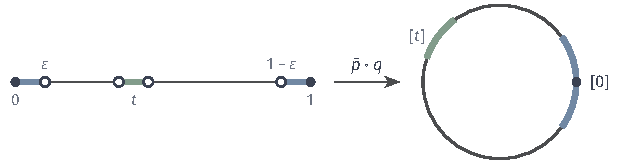
\includegraphics[width=105.11mm]{figures/04-spaces-measures-and-geometry/01-topology-and-metric/tikz/topo-quotient-circle/figure.pdf}
  \caption{区间端点粘合成圆，图中$\varepsilon=0.1$，$t=0.4$。蓝色的两段$[0,\varepsilon)$与$(1-\varepsilon,1]$在粘合后接成粘合点$[0]$的一段开邻域；绿色的小区间对应内部点$[t]$的开邻域。}
  \label{fig:topo-quotient-circle}
\end{BookInlineFigure}

\paragraph{从商空间出发的映射}
商空间上的映射通常是这样得到的：先在$X$上写出一个映射，再检验它在每个等价类上取同一个值。连续性则可以回到$X$上判断。

\begin{theorem}[商空间上的映射]
\label{thm:topo-quotient-maps}
设$q:X\to X/{\sim}$为商映射，$Z$为拓扑空间。
\begin{enumerate}
  \item 映射$g:X/{\sim}\to Z$连续，当且仅当$g\circ q:X\to Z$连续；
  \item 若$f:X\to Z$连续，并且$x\sim y$时$f(x)=f(y)$，则存在唯一的连续映射$\bar f:X/{\sim}\to Z$使$\bar f\circ q=f$。
\end{enumerate}
\end{theorem}
\begin{proof}
对$Z$的开集$W$，有
\[
 q^{-1}\bigl(g^{-1}(W)\bigr)=(g\circ q)^{-1}(W).
\]
按商拓扑的定义，$g^{-1}(W)$开当且仅当左边开，第一条成立。

对第二条，令$\bar f([x])=f(x)$。$f$在每个类上取同一个值，所以这个定义不依赖代表元的选择，并且$\bar f\circ q=f$。$q$是满射，满足这个等式的映射只能是$\bar f$。由$\bar f\circ q=f$连续及第一条，$\bar f$连续。
\end{proof}

把定理用于例~\ref{ex:topo-interval-gluing-circle}：$p:I\to S^1$连续且$p(0)=p(1)$，于是诱导出连续映射$\bar p:I/{\sim}\to S^1$。$p$在$(0,1)$上单射，并且只有$0,1$两点映到$(1,0)$，所以$\bar p$是双射。

到这里得到的只是连续双射。要说明$\bar p^{-1}$也连续，还需要关于紧性和分离性的工具，第~\ref{sec:topo-compact-images}小节完成这一步。另一方面，粘合可能破坏“不同点能用开集分开”这一性质，第~\ref{sec:topo-separation}小节会给出这样的商空间。


\section{空间的性质}
\label{sec:topo-properties}

前几节的例子显示，拓扑空间可以离日常的几何直觉很远：平凡拓扑中所有点都挤在一起，点列同时收敛到每个点；余可数拓扑中点列几乎探测不到闭包。本节集中研究整个空间满足的几类条件，它们排除这些病态现象，或者保证局部信息能够汇成整体信息。分离性问不同点能否被邻域分开；可数性与可分性问开集、邻域和稠密点集能否用可数个代表描述；连通性问空间能否拆成两块；紧性问开覆盖能否化为有限个。每项条件都用前面的点列、映射与构造来检验它的后果。

\subsection{分离性}
\label{sec:topo-separation}

在$\mathbb R$中，两个不同的点$x<y$可以分别放进$(x-r,x+r)$与$(y-r,y+r)$，其中$r=(y-x)/2$，两个区间不相交。平凡拓扑中做不到这一点，因为每个点的唯一开邻域都是全空间；正是这个缺陷让点列在平凡拓扑中有多个极限。

\begin{definition}[Hausdorff空间]
\label{def:topo-hausdorff}
若对$X$中任意两个不同的点$x\neq y$，都存在开集$U\ni x$与$V\ni y$使$U\cap V=\varnothing$，就称$X$为\term{Hausdorff空间}（Hausdorff space）。
\end{definition}

$\mathbb R$是Hausdorff空间。$\mathbb R^n$也是：若$\bm x\neq\bm y$，它们至少有一个坐标不同，设$x_i\neq y_i$，在第$i$个坐标上取两个不交的开区间，其余坐标取$\mathbb R$，得到两个不交的开矩形。这个论证对一般情形同样适用：两个Hausdorff空间的乘积仍是Hausdorff空间，因为两点在某个因子中不同，就在那个因子中分开。Hausdorff空间的子空间也是Hausdorff空间：若$U,V$在$X$中分开$x,y\in A$，则$U\cap A$与$V\cap A$在$A$中分开它们。所以平面上的圆周、曲线和区域都是Hausdorff空间。

\paragraph{极限的唯一性}
分离条件直接解决了第~\ref{sec:topo-convergence}节留下的极限唯一性问题。

\begin{theorem}[Hausdorff空间中极限唯一]
\label{thm:topo-hausdorff-unique-limit}
在Hausdorff空间中，每个收敛点列只有一个极限。
\end{theorem}
\begin{proof}
设$x_n\to x$且$x_n\to y$，$x\neq y$。取不交的开集$U\ni x$，$V\ni y$。存在$n_1$使$n\geq n_1$时$x_n\in U$，存在$n_2$使$n\geq n_2$时$x_n\in V$。取$n=\max\{n_1,n_2\}$，则$x_n\in U\cap V=\varnothing$，矛盾。
\end{proof}

因此在Hausdorff空间中可以写$\lim_{n\to\infty}x_n=x$。这个定理只需要两个邻域不交；它不要求空间有距离，也不需要可数性。

\paragraph{商空间是否仍可分离}
子空间与乘积保持Hausdorff性质，商空间则不一定，需要逐个检查。先看例~\ref{ex:topo-interval-gluing-circle}的商空间$I/{\sim}$（$0\sim1$）。两个内部点$[s]\neq[t]$（$0<s<t<1$）可以用$(0,1)$中两个不交小区间的像分开，这些像是开集，因为它们的原像就是这两个小区间。内部点$[t]$与粘合点$[0]$之间，取$\varepsilon<\min\{t,1-t\}/2$，用$(t-\varepsilon,t+\varepsilon)$的像与$[0,\varepsilon)\cup(1-\varepsilon,1]$的像分开；后者的原像正是这个并集，所以是开集。于是$I/{\sim}$是Hausdorff空间。

\begin{example}[有两个原点的直线]
\label{ex:topo-line-two-origins}
取两条实轴的并$X=\mathbb R\times\{0,1\}$（$\{0,1\}$取离散拓扑，$X$取乘积拓扑），对每个$t\neq0$令$(t,0)\sim(t,1)$，其余点只与自身等价。商空间$X/{\sim}$看起来像一条实轴，只是原点处有两个点$o_0=[(0,0)]$与$o_1=[(0,1)]$。

这两个原点不能被分开。设$V_0\ni o_0$、$V_1\ni o_1$是开集，则$q^{-1}(V_0)$是含$(0,0)$的开集，包含某个$(-\varepsilon,\varepsilon)\times\{0\}$；同样$q^{-1}(V_1)$包含某个$(-\varepsilon',\varepsilon')\times\{1\}$。取$0<t<\min\{\varepsilon,\varepsilon'\}$，则$[(t,0)]=[(t,1)]$同时属于$V_0$与$V_1$，所以二者相交。由此$X/{\sim}$不是Hausdorff空间，点列$[(1/n,0)]$同时收敛到$o_0$与$o_1$。
\end{example}

这个例子的每一点附近都像实轴的一段，局部看不出任何问题，整体却失去了极限唯一性。所以定义流形时，“局部像欧氏空间”之外还要单独要求Hausdorff条件，见第~\ref{chap:manifold-basics}章。

\subsection{可数性}
\label{sec:topo-countability}

$\mathbb R$有不可数个点，开集更多，但第~\ref{sec:topo-neighborhood-basis}小节已经看到，一个点的全部邻域可以由可数个区间$(x-1/k,x+1/k)$代表。类似地，全部开集能否由可数个基本开集生成？这两个问题分别针对一个点的邻域族和整个空间的开集族。

\begin{definition}[第一可数与第二可数]
\label{def:topo-countability}
若$X$的每个点都有一个可数的邻域基，称$X$\term{第一可数}（first countable）。若$X$有一个可数的拓扑基，称$X$\term{第二可数}（second countable）。
\end{definition}

这里“可数”包括有限。第一可数是逐点的条件，不同点的邻域基可以毫无关系；第二可数是整体的条件，要求一族可数的开集同时服务于所有点。由引理~\ref{lem:topo-basis-to-neighborhood-basis}，从可数拓扑基中取出含$x$的成员，就得到$x$的可数邻域基，所以第二可数蕴含第一可数。

\begin{example}[有理端点区间]
\label{ex:topo-rational-intervals}
在$\mathbb R$中，令$\mathcal B_{\mathbb Q}=\{(p,q):p,q\in\mathbb Q,\ p<q\}$。它是可数集，因为它与$\mathbb Q\times\mathbb Q$的一个子集一一对应，而可数集的有限乘积可数，可参考\BookChapterRef{chap:cardinality}{卷一第3章“基数”}。它是拓扑基：设$U$开，$x\in U$，取$r>0$使$(x-r,x+r)\subseteq U$，由$\mathbb Q$的稠密性取有理数$p\in(x-r,x)$与$q\in(x,x+r)$，则$x\in(p,q)\subseteq U$。

所以$\mathbb R$第二可数。同理，有理端点的开矩形$(p_1,q_1)\times\cdots\times(p_n,q_n)$构成$\mathbb R^n$的可数拓扑基：给定开集$U\ni\bm x$，先取开矩形$\bm x\in R\subseteq U$，再在每个坐标上把区间缩小为含$x_i$的有理端点区间。由于$\mathbb R^n$有不可数个点，这些例子说明，可数性条件约束的是开集族与邻域族的规模，而不是点的个数。
\end{example}

另一方面，第一可数不能推出第二可数。设$X$是不可数集，取离散拓扑。每个点有一个只含一个成员的邻域基$\{\{x\}\}$，所以$X$第一可数。但任何拓扑基$\mathcal B$都必须包含每个单点集：开集$\{x\}$是$\mathcal B$中成员的并，而这些成员都非空且含于$\{x\}$，只能是$\{x\}$本身。于是$\mathcal B$不可数，$X$不第二可数。

第一可数性的意义在于让点列重新可用：若$x\in\overline A$且$x$有可数邻域基$N_1\supseteq N_2\supseteq\cdots$（必要时取前$k$个的交），从每个$N_k\cap A$中选一点，得到的点列就收敛到$x$。例~\ref{ex:topo-cocountable}的余可数拓扑不第一可数，所以点列在那里失效。度量空间都是第一可数的，相应的闭包与闭集序列判据在第~\ref{chap:metric-spaces}章展开。第二可数性则是流形定义中的另一项要求，它保证流形可以由可数个坐标区域拼成。

\subsection{可分性}
\label{sec:topo-separability}

可数性条件谈的是开集族，另一种“可数描述”谈的是点：能否找到可数个点，使它们接近空间中的每一点？在$\mathbb R$中，可数的$\mathbb Q$就做到了这一点，因而数值计算只用有理数也能逼近任何实数。

\begin{definition}[可分空间]
\label{def:topo-separable}
若$X$含有一个可数的稠密子集，称$X$为\term{可分}（separable）空间。
\end{definition}

由例~\ref{ex:topo-rationals-irrationals-dense}，$\mathbb R$是可分的，尽管它不可数；$\mathbb R^n$也可分，$\mathbb Q^n$是可数稠密子集，因为每个非空开集含一个开矩形，开矩形的每个坐标区间都含有理数。可分性与可数性一样，并不限制点的个数。

\paragraph{可分性取决于拓扑}
同一个集合换一个拓扑，可分性可能改变。设$X$是不可数集，取离散拓扑。若$D$稠密，由定理~\ref{thm:topo-dense-open-criterion}，每个非空开集$\{x\}$都与$D$相交，即$x\in D$，所以唯一的稠密子集是$X$本身。$X$不可数，因此不可分。同一个$\mathbb R$，通常拓扑下可分，离散拓扑下不可分；而在平凡拓扑下，任何非空子集都稠密，单点集就够了。

\paragraph{三种可数要求的区别}
到这里出现了三种“可数”：可数稠密点集、可数拓扑基、每点的可数邻域基。它们分别描述点、整体开集族和逐点邻域族，不能互相替代。第二可数能推出可分：在可数拓扑基的每个非空成员中各选一点，得到可数集$D$；每个非空开集都含某个非空基本开集，因而与$D$相交，$D$稠密。

反过来，可分且第一可数的空间也未必第二可数。在$\mathbb R$上以全体半开区间$[a,b)$为基生成拓扑，称为\term{Sorgenfrey直线}（Sorgenfrey line）；两个半开区间的交仍是半开区间或空集，定理~\ref{thm:topo-basis-criterion}的条件成立。每个$[a,b)$都含有理数，所以$\mathbb Q$稠密，空间可分；$\{[x,x+1/k)\}$是$x$的可数邻域基，空间第一可数。但若$\mathcal B$是任意拓扑基，对每个$x$，开集$[x,x+1)$含$x$，必有$B_x\in\mathcal B$使$x\in B_x\subseteq[x,x+1)$，于是$x=\min B_x$。不同的$x$给出不同的$B_x$，所以$\mathcal B$不可数。

在度量空间中，第二可数与可分是等价的，这一结论在第~\ref{chap:metric-spaces}章证明；Sorgenfrey直线说明这个等价依赖距离，并非一般拓扑空间的性质。

\subsection{连通性}
\label{sec:topo-connectedness}

区间$[0,1]$是“一整块”，而$[0,1]\cup[2,3]$由两块组成。描述这种区别有两种思路：一是问空间能否被分成两个互不接触的部分，二是问任意两点能否用一条连续曲线连起来。前者只用开集，称为连通；后者需要显式的路径，称为路径连通。下面分别讨论，并说明在什么局部条件下二者一致。

\subsubsection{连通集}
\label{sec:topo-connected-sets}

$[0,1]\cup[2,3]$可以写成两个不交的非空集合之并，并且每一块都不包含另一块的闭包点，因而两块在这个空间中都是开集。连通就是排除这种分解。

\begin{definition}[连通空间]
\label{def:topo-connected}
若$X$不能写成两个不交的非空开集之并，称$X$\term{连通}（connected）。子集$A\subseteq X$称为连通集，如果$A$作为子空间连通。
\end{definition}

若$X=U\cup V$，$U,V$不交且开，则$U=X\setminus V$也是闭集。所以$X$连通，当且仅当$X$中既开又闭的子集只有$\varnothing$与$X$。这就是第~\ref{sec:topo-closed-sets}小节所说的用途：只要找到一个非平凡的既开又闭子集，空间就被拆开了。离散拓扑下超过一点的空间不连通，平凡拓扑下的空间总是连通的。

\paragraph{实轴上的连通集}
实轴上“没有缺口”的集合是区间：若$x,y\in A$且$x<z<y$，则$z\in A$。下面的定理说明，连通正好刻画了这一点。

\begin{theorem}[实轴上的连通集]
\label{thm:topo-connected-intervals}
子集$A\subseteq\mathbb R$连通，当且仅当$A$是区间。
\end{theorem}
\begin{proof}
若$A$不是区间，存在$x,y\in A$与$z\notin A$，$x<z<y$。则$A=((-\infty,z)\cap A)\cup((z,\infty)\cap A)$，两部分在$A$中相对开、不交，并分别含$x$与$y$，$A$不连通。

设$A$是区间，假设$A=U\cup V$，$U,V$在$A$中相对开、不交且非空。取$a\in U$，$b\in V$，不妨设$a<b$，则$[a,b]\subseteq A$。令$s=\sup(U\cap[a,b])$，则$s\in[a,b]\subseteq A$，下面说明$s$既不能在$U$中，也不能在$V$中。

若$s\in U$，则$s\neq b$，即$s<b$。$U$相对开，存在$\varepsilon>0$使$(s-\varepsilon,s+\varepsilon)\cap A\subseteq U$，于是$(s,\min\{s+\varepsilon,b\})$中的点属于$U\cap[a,b]$，且大于$s$，与上确界的定义矛盾。若$s\in V$，则$s\neq a$，即$s>a$，同样有$\varepsilon>0$使$(s-\varepsilon,s]\cap[a,b]\subseteq V$；这些点都不属于$U$，所以$U\cap[a,b]$中的点都不超过$s-\varepsilon$，与$s$是最小上界矛盾。
\end{proof}

所以$(0,1)$、$[0,1]$、$\mathbb R$都连通，而$(0,1)\cup(2,3)$不连通。证明中用到的是实数的确界原理，这正是“实轴没有缺口”的数学表述；在$\mathbb Q$中同样的论证失败，下文会看到$\mathbb Q$确实不连通。

\paragraph{连续像与介值}
连通性是只用开集表述的性质，连续映射通过原像把开集的分解拉回定义域，因此不能凭空制造分解。

\begin{theorem}[连通集的连续像]
\label{thm:topo-connected-image}
设$f:X\to Y$连续，$X$连通，则$f(X)$连通。
\end{theorem}
\begin{proof}
把$f$看成$X\to f(X)$的映射，由引理~\ref{lem:topo-map-into-subspace}它仍连续。若$f(X)=U\cup V$，$U,V$在$f(X)$中不交、开、非空，则$X=f^{-1}(U)\cup f^{-1}(V)$，两个原像开、不交，且因为$U,V$含有像点而非空，与$X$连通矛盾。
\end{proof}

与定理~\ref{thm:topo-connected-intervals}结合，就得到介值定理的一般形式：若$X$连通，$f:X\to\mathbb R$连续，则$f(X)$是区间；因此若$f$取到值$a<b$，它也取到$a,b$之间的每个值。特别地，同胚保持连通性，所以$[0,1)$与$(0,1)\cup(2,3)$不同胚。

\paragraph{连通分支}
不连通的空间可以分成若干“最大的连通块”。为此需要两个引理，说明连通集在什么情况下合并或扩大后仍连通。

\begin{lemma}[连通集的并与闭包]
\label{lem:topo-connected-union-closure}
\begin{enumerate}
  \item 若一族连通子集$A_i$（$i\in I$）有公共点$p$，则$\bigcup_iA_i$连通；
  \item 若$A$连通，且$A\subseteq B\subseteq\overline A$，则$B$连通。特别地，$\overline A$连通。
\end{enumerate}
\end{lemma}
\begin{proof}
记$S=\bigcup_iA_i$，设$S=U\cup V$，$U,V$在$S$中不交、相对开，不妨$p\in U$。对每个$i$，$A_i\cap U$与$A_i\cap V$在$A_i$中相对开、不交，并覆盖$A_i$；$A_i$连通且$p\in A_i\cap U$，所以$A_i\cap V=\varnothing$，即$A_i\subseteq U$。于是$S\subseteq U$，$V=\varnothing$，第一条成立。

对第二条，设$B=U\cup V$为$B$中不交、相对开的分解。同上，$A$连通，所以$A$整个落在其中一块，不妨$A\subseteq U$。若$V$非空，取$v\in V$，写$V=V'\cap B$，$V'$为$X$的开集。$V'$是$v$的邻域而$v\in\overline A$，所以$V'$与$A$相交；交点属于$A\cap V'\subseteq B\cap V'=V$，与$A\subseteq U$矛盾。故$V=\varnothing$。
\end{proof}

对$x\in X$，令$C(x)$为所有含$x$的连通子集之并。由引理第一条，$C(x)$连通，并且它是含$x$的最大连通子集，称为$x$所在的\term{连通分支}（connected component）。若$C(x)$与$C(y)$相交，二者之并连通且含$x$，由最大性等于$C(x)$，同理等于$C(y)$；所以连通分支两两不交，构成$X$的一个划分。由引理第二条，$\overline{C(x)}$也是含$x$的连通集，故$\overline{C(x)}=C(x)$，连通分支总是闭集。

\begin{example}[连通分支]
\label{ex:topo-components}
$(0,1)\cup(2,3)$的连通分支是$(0,1)$与$(2,3)$。$\mathbb Q$的连通分支是全部单点集：若$A\subseteq\mathbb Q$含两个有理数$p<q$，取无理数$z\in(p,q)$，$(-\infty,z)\cap A$与$(z,\infty)\cap A$就把$A$分开。单点集在$\mathbb Q$中不是开集，所以连通分支一般只是闭集，不必是开集。
\end{example}

\subsubsection{路径连通性}
\label{sec:topo-path-connected}

连通性告诉我们空间不能被拆开，却没有给出从一点到另一点的具体方式。在平面区域中，我们更习惯用一条曲线把两点连起来。下面把“曲线”定义为区间的连续像。

\begin{definition}[路径与路径连通]
\label{def:topo-path-connected}
设$I=[0,1]$。连续映射$\gamma:I\to X$称为从$\gamma(0)$到$\gamma(1)$的\term{路径}（path）。若$X$中任意两点之间都有路径，称$X$\term{路径连通}（path-connected）。
\end{definition}

在$\mathbb R^n$中，线段$\gamma(t)=(1-t)\bm a+t\bm b$是从$\bm a$到$\bm b$的路径，由逐坐标判据它连续；所以$\mathbb R^n$本身、开矩形、开圆盘以及一切凸集都路径连通。

\paragraph{路径分支}
“$x$与$y$之间有路径”是$X$上的等价关系。自反性用常值路径；对称性用反向路径$\bar\gamma(t)=\gamma(1-t)$。传递性需要把从$x$到$y$的路径$\alpha$与从$y$到$z$的路径$\beta$接起来：
\begin{equation}
(\alpha\cdot\beta)(t)=
\begin{cases}
\alpha(2t), & 0\leq t\leq 1/2,\\
\beta(2t-1), & 1/2\leq t\leq 1.
\end{cases}
\label{eq:topo-path-concatenation}
\end{equation}
在$t=1/2$处两段都给出$y$，所以定义无歧义。它的连续性来自下面的粘接引理：若$X=F_1\cup F_2$，$F_1,F_2$闭，$f$在每个$F_j$上的限制连续，则$f$连续。证明只需看闭集$C$的原像：$f^{-1}(C)=(f|_{F_1})^{-1}(C)\cup(f|_{F_2})^{-1}(C)$，每一部分在$F_j$中相对闭，因而形如$F_j$与闭集之交，在$X$中闭。

这个等价关系的等价类称为\term{路径分支}（path component）。路径连通的空间只有一个路径分支。

\paragraph{路径连通蕴含连通}
路径的像是区间$I$的连续像，由定理~\ref{thm:topo-connected-intervals}与定理~\ref{thm:topo-connected-image}是连通集。因此路径连通的空间一定连通：固定$x_0\in X$，对每个$y$取一条从$x_0$到$y$的路径$\gamma_y$，则$X=\bigcup_y\gamma_y(I)$，这些连通集有公共点$x_0$，由引理~\ref{lem:topo-connected-union-closure}，$X$连通。同理，每个路径分支都含于某个连通分支。

\begin{example}[连通但不路径连通]
\label{ex:topo-topologist-sine}
在$\mathbb R^2$中令$G=\{(x,\sin(1/x)):0<x\leq1\}$，$J=\{0\}\times[-1,1]$，$S=G\cup J$。$G$是区间$(0,1]$在连续映射$x\mapsto(x,\sin(1/x))$下的像，因而连通。对$(0,y)\in J$，取$\theta$使$\sin\theta=y$，则$x_k=1/(\theta+2k\pi)\to0$（$k$充分大时$x_k\in(0,1]$），而$(x_k,y)\in G$收敛到$(0,y)$，由定理~\ref{thm:topo-subsequence-closure}，$J\subseteq\overline G$。于是$G\subseteq S\subseteq\overline G$，由引理~\ref{lem:topo-connected-union-closure}，$S$连通。

但没有路径从$(0,0)$连到$(1,\sin1)$。假设$\gamma=(\gamma_1,\gamma_2):I\to S$是这样的路径。$T=\gamma_1^{-1}(\{0\})$是闭集，含$0$而不含$1$，令$t_0=\max T<1$。当$t>t_0$时$\gamma(t)\in G$，所以$\gamma_2(t)=\sin(1/\gamma_1(t))$。由$\gamma_2$在$t_0$处连续，取$\delta\in(0,1-t_0]$使$t\in[t_0,t_0+\delta]$时$\lvert\gamma_2(t)-\gamma_2(t_0)\rvert<1/2$。

记$a=\gamma_1(t_0+\delta)>0$。$\gamma_1$在$[t_0,t_0+\delta]$上从$0$连续变到$a$，由介值定理取遍$(0,a]$。取正整数$k$使$x^+=1/(\pi/2+2k\pi)$与$x^-=1/(3\pi/2+2k\pi)$都小于$a$，则有$t^\pm\in(t_0,t_0+\delta]$使$\gamma_1(t^\pm)=x^\pm$，相应地$\gamma_2(t^+)=1$，$\gamma_2(t^-)=-1$。这两个值相差$2$，却都与$\gamma_2(t_0)$相差小于$1/2$，矛盾。
\end{example}

集合$S$常称为拓扑学家的正弦曲线（topologist's sine curve）。它的问题出在$J$附近：$G$在$J$旁边无限次上下振荡，任何一个小邻域都把$S$切成无穷多段，路径无法在有限时间内穿过。排除这种局部现象，就能让连通与路径连通一致。

\paragraph{局部路径连通}
若对每个$x\in X$及$x$的每个邻域$N$，都存在路径连通的开集$V$使$x\in V\subseteq N$，称$X$\term{局部路径连通}（locally path-connected）。$\mathbb R^n$的开子集都局部路径连通：$\bm x$的邻域含一个以$\bm x$为中心的开矩形，开矩形是凸集，因而路径连通。

\begin{theorem}[局部路径连通时两种分支一致]
\label{thm:topo-locally-path-connected}
设$X$局部路径连通，则$X$的每个路径分支是开集，且路径分支与连通分支相同。特别地，连通且局部路径连通的空间是路径连通的。
\end{theorem}
\begin{proof}
设$P$是一个路径分支，$x\in P$。取路径连通的开集$V\ni x$，$V$中每点经$V$内的路径与$x$相连，所以$V\subseteq P$。于是$P$是开集。$X\setminus P$是其余路径分支之并，也是开集，所以$P$既开又闭。

设$C$是含$P$的连通分支（$P$连通，故含于一个连通分支）。$P\cap C=P$在$C$中既相对开又相对闭，且非空，由$C$连通得$P=C$。最后一句是$X$只有一个连通分支的情形。
\end{proof}

于是$\mathbb R^n$中连通的开集都是路径连通的，连通性可以用画出一条曲线来核验。例~\ref{ex:topo-topologist-sine}中的$S$在$J$上的点处不局部路径连通，定理的条件不满足。流形在每点附近同胚于欧氏空间的开集，因而局部路径连通，第~\ref{chap:manifold-basics}章将用这一点把流形的连通与路径连通等同起来。

\subsection{紧性}
\label{sec:topo-compactness}

闭区间上的连续函数有最大值，开区间上则未必；卷一把这一区别归结为闭区间的“有限子覆盖”性质。这个性质只用开集表述，因此可以搬到任何拓扑空间：它要求无论用什么方式以局部区域覆盖整个对象，都只需其中有限个。本小节先给出定义，再讨论闭包紧的集合，最后说明连续映射怎样保持紧性。

\subsubsection{紧性的定义}
\label{sec:topo-compact-definition}

一族开集$\{U_i\}_{i\in I}$若满足$\bigcup_iU_i=X$，称为$X$的\term{开覆盖}（open cover）；从中选出的、仍覆盖$X$的子族称为子覆盖，有限个成员组成的子覆盖称为\term{有限子覆盖}（finite subcover）。

\begin{definition}[紧空间与紧集]
\label{def:topo-compact}
若$X$的每个开覆盖都有有限子覆盖，称$X$\term{紧致}（compact），也称紧空间。子集$K\subseteq X$称为紧集，如果$K$作为子空间是紧的。
\end{definition}

子空间的开集是$U\cap K$的形式，所以$K$是紧集，当且仅当每一族满足$K\subseteq\bigcup_iU_i$的$X$的开集都有有限个成员仍覆盖$K$。以后检验紧集时直接用环境空间的开集，不必先转成相对开集。

\paragraph{某一个覆盖与所有覆盖}
定义中的量词是“每个开覆盖”。$(0,1)$有一个只含一个成员的开覆盖$\{(0,1)\}$，这不说明任何问题。考虑覆盖$\{(1/n,1):n\geq2\}$：每点$x\in(0,1)$在$n>1/x$时属于$(1/n,1)$，所以它覆盖$(0,1)$；但有限个成员之并是$(1/N,1)$，漏掉了$(0,1/N]$。所以$(0,1)$不紧。同理，$\{(-n,n):n\geq1\}$说明$\mathbb R$不紧。

闭区间$[a,b]$则是紧集，卷一已经用共同半径的论证证明了这一点。由下面的引理，$\mathbb R$中有界闭集都是紧集：它是某个$[a,b]$的闭子集。

\begin{lemma}[紧空间的闭子集]
\label{lem:topo-closed-in-compact}
紧空间$X$的闭子集$F$是紧集。
\end{lemma}
\begin{proof}
设$\{U_i\}$是$X$的开集，覆盖$F$。加上开集$X\setminus F$，得到$X$的开覆盖，取出有限子覆盖。去掉其中的$X\setminus F$（若出现），剩下的有限个$U_i$仍覆盖$F$。
\end{proof}

其他例子：有限集总是紧的，因为每点只需选一个含它的成员。无限集取离散拓扑时不紧，单点集组成的开覆盖没有有限子覆盖。平凡拓扑下的空间总是紧的，因为唯一的非空开集就是全空间。最后一例也说明，紧性本身不要求点能被分开。

在实轴上，紧性还可以用“每个点列有收敛子列”来刻画，卷一的证明正是在两种说法之间往返。一般拓扑空间中，两种说法可以不等价，点列也未必能探测拓扑，所以紧性以开覆盖定义。在度量空间中二者等价，并且紧等价于完备且全有界，这些判据在第~\ref{chap:metric-spaces}章建立。

\subsubsection{相对紧集}
\label{sec:topo-relatively-compact}

$(0,1)$本身不紧，但它离紧只差端点：补上闭包点后得到$[0,1]$，是紧集。很多估计只需要集合落在某个紧集里，而不需要集合本身紧，这引出下面的概念。

\begin{definition}[相对紧集]
\label{def:topo-relatively-compact}
设$A\subseteq X$。若$A$在$X$中的闭包$\overline A$是紧集，称$A$在$X$中\term{相对紧}（relatively compact）。
\end{definition}

$(0,1)$在$\mathbb R$中相对紧，但它既不闭也不紧；所以相对紧是比紧弱的条件。$\mathbb R$的每个有界子集都相对紧，因为它的闭包是有界闭集。紧集是否一定相对紧，涉及紧集的闭包；在Hausdorff空间中，这个问题由下面的引理回答。

\begin{lemma}[Hausdorff空间中的紧集是闭集]
\label{lem:topo-compact-closed-hausdorff}
设$X$是Hausdorff空间，$K\subseteq X$是紧集，则$K$是闭集。
\end{lemma}
\begin{proof}
取$x\notin K$。对每个$y\in K$，由Hausdorff条件取不交的开集$U_y\ni x$与$V_y\ni y$。$\{V_y\}_{y\in K}$覆盖$K$，取有限个$V_{y_1},\dots,V_{y_m}$覆盖$K$。则$U=U_{y_1}\cap\cdots\cap U_{y_m}$是含$x$的开集，与$V_{y_1}\cup\cdots\cup V_{y_m}\supseteq K$不交。所以$X\setminus K$是它每个点的邻域，是开集。
\end{proof}

由此，在Hausdorff空间中，紧集等于自己的闭包，因而相对紧；任何含于紧集$K$的子集$A$也相对紧，因为$\overline A$是$K$的闭子集，由引理~\ref{lem:topo-closed-in-compact}紧。没有Hausdorff条件时引理可以失效：平凡拓扑下超过一点的空间里，每个单点集都紧，却不闭。

\paragraph{相对紧依赖环境空间}
同一个集合在不同的环境中可能一个相对紧、一个不相对紧。把$(0,1)$看作空间$X=(0,1)$自身的子集，它在$X$中的闭包就是$X$，而$X$不紧，所以$(0,1)$在$(0,1)$中不相对紧；在$\mathbb R$中，它的闭包多了两个端点，成了紧集。这说明相对紧描述的是集合与环境的关系：环境中是否有足够的点让集合“收拢”。在度量空间中，相对紧可以用点列判据与全有界性来检验，这留到第~\ref{chap:metric-spaces}章。

\subsubsection{紧集的连续像}
\label{sec:topo-compact-images}

闭区间上连续函数取到最大值，这一结论的拓扑核心是：连续映射把紧集映成紧集，而实轴上的紧集有最大元。

\begin{theorem}[紧集的连续像]
\label{thm:topo-compact-image}
设$f:X\to Y$连续，$K\subseteq X$是紧集，则$f(K)$是$Y$中的紧集。
\end{theorem}
\begin{proof}
设$\{V_i\}$是$Y$的开集，覆盖$f(K)$。则$\{f^{-1}(V_i)\}$是$X$的开集，覆盖$K$：每个$x\in K$的像$f(x)$属于某个$V_i$。由$K$紧，取有限个$f^{-1}(V_{i_1}),\dots,f^{-1}(V_{i_m})$覆盖$K$，则$V_{i_1},\dots,V_{i_m}$覆盖$f(K)$。
\end{proof}

证明的方向值得注意：开覆盖在输出空间给出，经连续性拉回到输入空间，在那里用紧性有限化，再推回输出空间。连续性负责“拉回后仍是开覆盖”，紧性负责“有限化”，二者缺一不可。

\begin{theorem}[最大值与最小值]
\label{thm:topo-extreme-values}
设$K$是非空紧空间，$f:K\to\mathbb R$连续，则$f$有界，并且取到最大值与最小值。
\end{theorem}
\begin{proof}
由定理~\ref{thm:topo-compact-image}，$f(K)$是$\mathbb R$中的非空紧集。开区间$(-n,n)$（$n\geq1$）覆盖$f(K)$，有限个就够，所以$f(K)$含于某个$(-n,n)$，$f$有界。$\mathbb R$是Hausdorff空间，由引理~\ref{lem:topo-compact-closed-hausdorff}，$f(K)$是闭集。令$M=\sup f(K)$，对每个$\varepsilon>0$，$(M-\varepsilon,M+\varepsilon)$含$f(K)$中的点，所以$M\in\overline{f(K)}=f(K)$，即最大值$M$被取到。对$-f$用同样的论证得到最小值。
\end{proof}

两个条件都不能去掉。$f(x)=x$在$(0,1)$上连续，但$(0,1)$不紧，$f$没有最大值。在紧集$[0,1]$上，令$f(x)=x$（$x<1$）且$f(1)=0$，则$f$不连续，上确界$1$取不到。

\paragraph{同胚保持紧性}
若$h:X\to Y$是同胚，$X$紧，则$Y=h(X)$紧；反过来用$h^{-1}$。所以紧性与连通性一样是拓扑性质。由此，$[0,1]$与$(0,1)$不同胚，尽管二者都连通。紧性还给出判断同胚的一个有力工具，它回答了第~\ref{sec:topo-quotients}小节留下的问题。

\begin{theorem}[从紧空间到Hausdorff空间的连续双射]
\label{thm:topo-compact-hausdorff-homeomorphism}
设$X$紧，$Y$是Hausdorff空间，$f:X\to Y$是连续双射，则$f$是同胚。
\end{theorem}
\begin{proof}
只需证明$f^{-1}$连续，由定理~\ref{thm:topo-continuity-equivalent}，即证明$f$把$X$的闭集映成闭集，因为$(f^{-1})^{-1}(F)=f(F)$。设$F$在$X$中闭，由引理~\ref{lem:topo-closed-in-compact}，$F$紧；由定理~\ref{thm:topo-compact-image}，$f(F)$紧；由引理~\ref{lem:topo-compact-closed-hausdorff}，$f(F)$在$Y$中闭。
\end{proof}

现在回到例~\ref{ex:topo-interval-gluing-circle}。商空间$I/{\sim}=q(I)$是紧集$I$的连续像，因而紧；$S^1$是Hausdorff空间$\mathbb R^2$的子空间，因而是Hausdorff空间。所以连续双射$\bar p:I/{\sim}\to S^1$是同胚，“把线段两端粘起来”确实得到圆周。对照例~\ref{ex:topo-interval-to-circle}，$[0,1)\to S^1$同样是连续双射，却不是同胚；定理在那里不适用，因为$[0,1)$不紧。


\section{本章小结}
\label{sec:topo-summary}

章首问的是：没有距离时，怎样谈论“附近”“趋于”和“连续”。本章的回答是把开集族作为唯一的基本数据。实轴开集满足的三条规则（空集与全空间开，任意并开，有限交开）被取作拓扑的定义；拓扑基用并生成全部开集，邻域与邻域基则只描述一个点周围的区域。离散拓扑、平凡拓扑和余可数拓扑表明，同一集合上的不同拓扑会给出截然不同的“附近”。

在固定的拓扑下，子集与环境的关系由闭集、内部、闭包与边界描述，它们都由邻域判据定义，并随拓扑改变；稠密集是闭包为全空间的集合，等价于与每个非空开集相交。点列收敛要求点列最终落入极限的每个邻域，收敛点列的子列收敛到同一点，闭集留住已有的极限；但余可数拓扑的例子说明，一般空间中点列不能反推闭包，因此闭包与稠密性都不以点列定义。

映射的连续性由开集的原像为开集来定义，等价于逐点的邻域判据与闭集原像判据，并保持点列极限，反过来的序列判据需要额外条件。开映射约束的是像，与连续性互不蕴含；同胚是双向连续的双射，连续双射为同胚当且仅当它是开映射。$(-1,1)$与$\mathbb R$同胚表明，拓扑不记录长度和有界性。子空间、有限乘积与商空间分别使包含映射、坐标投影与商映射连续，并给出映入子空间与乘积、映出商空间的连续性判据；$X\times[0,1]$是同伦的定义域，区间端点的粘合给出圆周。

空间的性质中，Hausdorff条件保证极限唯一，子空间与乘积保持它，商空间则可能破坏它，有两个原点的直线就是例子。第二可数是整体开集族的可数性，第一可数是逐点邻域族的可数性，可分是可数稠密点集的存在性，三者都不限制点的个数；第二可数蕴含另外两者，Sorgenfrey直线说明反向一般不成立。连通性只用开集表述，实轴上的连通集恰为区间，连续像保持连通并推出介值定理；路径连通蕴含连通，拓扑学家的正弦曲线说明反向不成立，局部路径连通时两种分支一致。紧性要求每个开覆盖都可有限化，连续像保持紧性，由此得到最值定理；从紧空间到Hausdorff空间的连续双射是同胚，这证明了区间粘合确实得到圆周。

本章所有概念都不依赖距离，这也划定了它的边界。距离会带来更多结构：闭包可用点到集合的距离刻画，第二可数与可分等价，紧性可用序列紧与“完备且全有界”判断，这些是第~\ref{chap:metric-spaces}章的内容；连续性的距离判据、均匀连续与映射列的收敛在第~\ref{chap:metric-space-maps}章讨论。另一方面，连续变形保留什么信息，要借助本章的乘积与商构造，在第~\ref{chap:homology}章用同调来回答。

